% Enable warnings on deprecated things.
\RequirePackage[l2tabu, orthodox]{nag}

\documentclass{scrreprt}

% Load custom packages+settings and commands.
%\usepackage{algorithm}
\usepackage[algochapter,noline,linesnumbered]{algorithm2e}
\DontPrintSemicolon
\SetKwProg{Fn}{Function}{ is}{end}
\SetKw{call}{call}
\newcommand{\forcond}{$i=0$ \KwTo $n$}
\SetKwFunction{Reach}{Reachability}%
\usepackage{algorithmicx}
\usepackage[noend]{algpseudocode}
\usepackage{style_and_commands/style}
\usepackage{color}
\usepackage{subcaption}
\usepackage{enumitem}
\usepackage[]{algorithm2e}
\usepackage{pdflscape}
\usepackage{tabularx}
% \usepackage{lscape}
\setitemize{noitemsep,topsep=0pt,parsep=0pt,partopsep=0pt}
% Project related.
  % Project information.
  \newcommand{\projecttitle}{ANOM: A(nother) step forward for aSTEP}
  \newcommand{\projectsubtitle}{Anomaly detection with a Neural network On Multivariate time series data}
 
  \newcommand{\projecttheme}{Developing Complex Software Systems}
  \newcommand{\projekttema}{Indlejret Systemer}
  \newcommand{\projectperiod}{Spring semester 2020}
  \newcommand{\projektperiode}{Efterårssemester 2019}
  %\newcommand{\projectcopies}{}
  \newcommand{\projectcompletion}{May 28th 2020}
  \newcommand{\projektaflevering}{19. december 2019}

  % Names.
  \newcommand{\groupname}{SW604F20}
  \newcommand{\supervisor}{Tung Kieu}
  \newcommand{\groupmembersbyfirstname}[0]{%
    Jeppe Andreas Arnfelt \newline
    Jonas Madsen \newline
    Kristian Otte \newline
    Kristian Simoni Vestermark \newline
    Rasmus Møller Jensen \newline
  }

% Custom styling commands.
  % Monospaced text.
  \newcommand*\justify{%
    \fontdimen2\font=0.4em% interword space
    \fontdimen3\font=0.2em% interword stretch
    \fontdimen4\font=0.1em% interword shrink
    \fontdimen7\font=0.1em% extra space
    \hyphenchar\font=`\-% allowing hyphenation
  }
  \newcommand{\mono}[1]{\texttt{\justify {#1}}}

  % Code mono
  \newcommand{\code}[1]{\sethlcolor{clcodeshade}\hl{\texttt{\justify{#1}}}} % Yes, this line is identical to the one in \mono, however the soul-package is fragile, and cannot see into another command.
  \soulregister{\justify}{1}

  % Chapter introductions.
  \newcommand{\chapterintro}[1]{#1}

  % CD paths with icon.
  %\newcommand{\cdpath}[1]{%
  %  % Param1: path
  %  \hyperref[app:cd]{\raisebox{-0.28ex}{\includegraphics[height=0.85em]{cd}}\mono{/#1}}%
  %}

  % Margin text.
  \newcommand{\margintext}[1]{\marginline{\textsf{\footnotesize #1}}}

  % Todo.
  \newcommand{\todo}[1]{\fxnote{#1}}

  % Dummy line.
  \newcommand{\dummy}{\usnote{Write an abstract here}}

% Document structure.
  % Sprints.

  % Document organization.
  \newenvironment{documentorganization}
    {\vspace{.5cm}\noindent\textbf{Report Organization}\quad The remainder of this report is organized in the following fashion:\begin{itemize}}
    {\end{itemize}}

  % Chapter organization.
  \newenvironment{chapterorganization}
    {\vspace{.5cm}\noindent\textbf{Chapter Organization}\quad This chapter is organized in the following fashion:\begin{itemize}}
    {\end{itemize}}

   % Abbreviation.
  \newenvironment{abbreviations}
    {\vspace{.5cm}\noindent\textbf{Chapter Abbreviations}\quad This chapter introduces the following abbreviations:\begin{addmargin}[\leftmargin]{0em}\begin{multicols}{2}\begin{description}[noitemsep, style=sameline]}
    {\end{description}\end{multicols}\end{addmargin}}

    % Dates.
    %\newenvironment{dates}
    %{\vspace{.5cm}\noindent\textbf{Project Dates}\quad \dummy:\begin{addmargin}[\leftmargin]{0em}\begin{multicols}{2}\begin{description}[noitemsep, style=sameline]}
    %{\end{description}\end{multicols}\end{addmargin}}

% Figures.
  % Normal figure.
  \newcommand{\fig}[3]{
    \begin{figure}[tbp]
      \centering
      %\rule{\textwidth}{0.005in}
      \includegraphics[width=0.75\textwidth]{#1}
      \caption[#2]{#3}\label{fig:#1}
      %\rule{\textwidth}{0.005in}
    \end{figure}
  }

  % Scaled figure.
  \newcommand{\figscaled}[4]{
    \begin{figure}[tbp]
      \centering
      \includegraphics[scale=#4]{#1}
      \caption[#2]{#3}\label{fig:#1}
    \end{figure}
  }

  % Figure with custom width.
  \newcommand{\figcustomwidth}[4]{
    \begin{figure}[tbp]
      \centering
      \includegraphics[width=#4]{#1}
      \caption[#2]{#3}\label{fig:#1}
    \end{figure}
  }

% References.
  \newcommand{\appendixref}[1]{\hyperref[#1]{Appendix \ref*{#1}}}
  \newcommand{\chapterref}[1]{\hyperref[#1]{Chapter \ref*{#1}}}
  \newcommand{\sectionref}[1]{\hyperref[#1]{Section \ref*{#1}}}
  \newcommand{\figureref}[1]{\hyperref[#1]{Figure \ref*{#1}}}
  \newcommand{\tableref}[1]{\hyperref[#1]{Table \ref*{#1}}}
  \newcommand{\listingref}[1]{\hyperref[#1]{Listing \ref*{#1}}}
  \newcommand{\onpage}[1]{on \hyperref[#1]{page \pageref*{#1}}}
  \newcommand{\equationref}[1]{\hyperref[#1]{Equation \ref*{#1}}}
  \newcommand{\algorithmref}[1]{\hyperref[#1]{Algorithm \ref*{#1}}}
  %\newcommand{\sprintref}[1]{\hyperref[#1]{Sprint \ref*{#1}}}

% Column types for tabulars.
%\newcolumntype{L}[1]{>{\raggedright\let\newline\\\arraybackslash\hspace{0pt}}m{#1}}
%\newcolumntype{R}[1]{>{\raggedleft\let\newline\\\arraybackslash\hspace{0pt}}m{#1}}

% Fix todo notes with externalize
\let\oldTodo\todo
\renewcommand{\todo}[1]{\tikzexternaldisable{}\oldTodo{#1}\tikzexternalenable{}}

% Fixme stuff.
%\newcommand{\fillin}[1]{\fxnote*[inline]{#1}{Fill in: }}

% Vector command.
%\newcommand{\omatrix}[1]{\ensuremath{\boldsymbol{#1}}}

% A better plus minus sign.
\makeatletter
\newcommand{\gpm}{\mathbin{\mathpalette\@gpm\relax}}
\newcommand{\@gpm}[2]{\ooalign{%
  \raisebox{.1\height}{$#1+$}\cr
  \smash{\raisebox{-.6\height}{$#1-$}}\cr}}
\makeatother


\definecolor{rosso}{RGB}{220,57,18}
\definecolor{giallo}{RGB}{255,153,0}
\definecolor{blu}{RGB}{102,140,217}
\definecolor{verde}{RGB}{16,150,24}
\definecolor{viola}{RGB}{153,0,153}

\makeatletter

\tikzstyle{chart}=[
    legend label/.style={font={\scriptsize},anchor=west,align=left},
    legend box/.style={rectangle, draw, minimum size=5pt},
    axis/.style={black,semithick,->},
    axis label/.style={anchor=east,font={\tiny}},
]

\tikzstyle{bar chart}=[
    chart,
    bar width/.code={
        \pgfmathparse{##1/2}
        \global\let\bar@w\pgfmathresult
    },
    bar/.style={very thick, draw=white},
    bar label/.style={font={\bf\small},anchor=north},
    bar value/.style={font={\footnotesize}},
    bar width=.75,
]

\tikzstyle{pie chart}=[
    chart,
    slice/.style={line cap=round, line join=round, very thick,draw=white},
    pie title/.style={font={\bf}},
    slice type/.style 2 args={
        ##1/.style={fill=##2},
        values of ##1/.style={}
    }
]

\pgfdeclarelayer{background}
\pgfdeclarelayer{foreground}
\pgfsetlayers{background,main,foreground}


\newcommand{\pie}[3][]{
    \begin{scope}[#1]
    \pgfmathsetmacro{\curA}{90}
    \pgfmathsetmacro{\r}{1}
    \def\c{(0,0)}
    \node[pie title] at (90:1.3) {#2};
    \foreach \v/\s in{#3}{
        \pgfmathsetmacro{\deltaA}{\v/100*360}
        \pgfmathsetmacro{\nextA}{\curA + \deltaA}
        \pgfmathsetmacro{\midA}{(\curA+\nextA)/2}

        \path[slice,\s] \c
            -- +(\curA:\r)
            arc (\curA:\nextA:\r)
            -- cycle;
        \pgfmathsetmacro{\d}{max((\deltaA * -(.5/50) + 1) , .5)}

        \begin{pgfonlayer}{foreground}
        \path \c -- node[pos=\d,pie values,values of \s]{$\v\%$} +(\midA:\r);
        \end{pgfonlayer}

        \global\let\curA\nextA
    }
    \end{scope}
}

\newcommand{\legend}[2][]{
    \begin{scope}[#1]
    \path
        \foreach \n/\s in {#2}
            {
                  ++(0,-10pt) node[\s,legend box] {} +(5pt,0) node[legend label] {\n}
            }
    ;
    \end{scope}
}

% each of the following has two versions
%   \crefname{environmentname}{singular}{plural}, to be used mid-sentence
%   \Crefname{environmentname}{singular}{plural}, to be used at the beginning of a sentence
\crefname{table}{table}{tables}
\Crefname{table}{Table}{Tables}
\crefname{figure}{figure}{figures}
\Crefname{figure}{Figure}{Figures}
\crefname{equation}{equation}{equations}
\Crefname{equation}{Equation}{Equations}


\let\URL\url
\makeatletter
\def\url#1{\@URL#1;;\@nil}
\def\@URL#1;#2;#3\@nil{%
  \URL{#1}\ifx\relax#2\relax\else; \URL{#2}\fi}
\makeatother

\newcommand\pro{\item[$+$]}
\newcommand\con{\item[$-$]}

% Vores egne
\let\oldsection\section
\renewcommand{\section}[1]{\FloatBarrier\oldsection{#1}}

% Set custom settings
  % Set true for PDF version ready for print. False for screen version.
  %\settoggle{printversion}{false}
  
  %To be deleted before hand-in!!!
  %\renewcommand{\includegraphics}[2][]{\rule{100pt}{70pt}}



% Set custom settings
  % Set true for PDF version ready for print. False for screen version.
  %\settoggle{printversion}{false}
  
  %To be deleted before hand-in!!!
  %\renewcommand{\includegraphics}[2][]{\rule{100pt}{70pt}}

\begin{document}
%\linenumbers

%Fixes for allowing more relaxed restrictions.
\footheight=20.4pt
\hbadness=99999
\tolerance=10000

 %Cover page.
\let\oldthepage\thepage{}
\renewcommand\thepage{Cover}
\bookmark[page=1,level=0]{Cover}
\tikzexternaldisable{}
%\includepdf[pages=-]{frontmatter/frontpage}
\tikzexternalenable{}
\renewcommand\thepage{\oldthepage}

%  A simple AAU report template.
%  2015-05-08 v. 1.2.0
%  Copyright 2010-2015 by Jesper Kjær Nielsen <jkn@es.aau.dk>
%
%  This is free software: you can redistribute it and/or modify
%  it under the terms of the GNU General Public License as published by
%  the Free Software Foundation, either version 3 of the License, or
%  (at your option) any later version.
%
%  This is distributed in the hope that it will be useful,
%  but WITHOUT ANY WARRANTY; without even the implied warranty of
%  MERCHANTABILITY or FITNESS FOR A PARTICULAR PURPOSE.  See the
%  GNU General Public License for more details.
%
%  You can find the GNU General Public License at <http://www.gnu.org/licenses/>.
%
\pdfbookmark[0]{Front page}{label:frontpage}%
\begin{titlepage}
  \addtolength{\hoffset}{0.5\evensidemargin-0.5\oddsidemargin} %set equal margins on the frontpage - remove this line if you want default margins
  \noindent%
  \begin{tabular}{@{}p{\textwidth}@{}}
    \toprule[2pt]
    \midrule
    \vspace{0.7cm}
    \begin{center}
    \Huge{\textbf{
    \projecttitle
    % insert your title here
    }}

    \end{center}
    \begin{center}
      \Large{
      \projectsubtitle
        % insert your subtitle here
      }
    \end{center}
    %\vspace{0.2cm}
    \\
    \midrule
    \toprule[2pt]
  \end{tabular}
  \vspace{4 cm}
  \begin{center}
    {\large
      Project Report%Insert document type (e.g., Project Report)
    }\\
    \vspace{0.2cm}
    {\Large
        \groupname %insert groupname or authors
    }
  \end{center}
  \vfill
  \begin{center}
  Aalborg University\\
  Department of Computer Science
  \end{center}
\end{titlepage}
\clearpage


\hypersetup{pageanchor=false} % To avoid problems with hyperref package
\thispagestyle{empty}
{\small
\strut\vfill
\noindent \copyright{} \groupname{} , Aalborg University, \MakeLowercase{\projectperiod{}}.\par
\vspace{0.3cm}
This report is set up using \LaTeX.


%\noindent Here you can write something about which tools and software you have used for typesetting the document, running simulations and creating figures. If you do not know what to write, either leave this page blank or have a look at the colophon in some of your books.\par
%\vspace{0.2cm}
}
\clearpage
\hypersetup{pageanchor=true} % Reenable this.

% Start roman numbering.
\cleardoublepage{}
\pagenumbering{roman}
\setcounter{page}{1}

\bookmark[page=3,level=0]{Title Page}
{
    %set up various length
    \ifx\titlepageleftcolumnwidth\undefined{}
      \newlength{\titlepageleftcolumnwidth}
      \newlength{\titlepagerightcolumnwidth}
    \fi
    \setlength{\titlepageleftcolumnwidth}{0.46\textwidth-\tabcolsep}
    \setlength{\titlepagerightcolumnwidth}{\textwidth-2\tabcolsep-\titlepageleftcolumnwidth}
    %create title page
    \thispagestyle{empty}
    \noindent%
    \begin{tabular}{@{}ll@{}}
      \parbox{0.97\titlepageleftcolumnwidth}{
          
\includegraphics[width=0.85\titlepageleftcolumnwidth]{Pictures/aau_logo_en.pdf}
      } &
      \vspace{1cm}
      \parbox{0.97\titlepagerightcolumnwidth}{\raggedleft\sffamily\small
        \textbf{\color{sectioning}Department of Computer Science}\\
        Selma Lagerlöfs Vej 300\\
        DK-9220 Aalborg Ø\\
        \href{http://www.cs.aau.dk}{http://www.cs.aau.dk/}
      }\bigskip\\
        \parbox[t]{\titlepageleftcolumnwidth}{
        \textbf{\color{sectioning}\sffamily{Title:}}\\ \projecttitle{}\bigskip\par
        \textbf{\color{sectioning}\sffamily{Theme:}}\\ \projecttheme{}\bigskip\par
        \textbf{\color{sectioning}\sffamily{Project period:}}\\ \projectperiod\bigskip\par
        \textbf{\color{sectioning}\sffamily{Project group:}}\\ \groupname{}\bigskip\par
        \textbf{\color{sectioning}\sffamily{Participant(s):}}\\ \groupmembersbyfirstname{}\bigskip\par
        \textbf{\color{sectioning}\sffamily{Supervisor(e):}}\\ \supervisor\bigskip\par
        %\textbf{\color{sectioning}\sffamily{Copies:}} \projectcopies\bigskip\par
        \textbf{\color{sectioning}\sffamily{Pages:}}~\pageref*{LastPageLabel}\bigskip\par
        \textbf{\color{sectioning}\sffamily{Total Pages:}} 5000\bigskip\par
        \textbf{\color{sectioning}\sffamily{Date of submission:}}\\ \projectcompletion
   } &
      \parbox[t]{0.97\titlepagerightcolumnwidth}{%
      \textbf{\color{sectioning}\sffamily{Abstract:}}\smallskip\par{}
        \fbox{\parbox{0.97\titlepagerightcolumnwidth-2\fboxsep-2\fboxrule}{%
          This project is part of the aSTEP project at AAU. It is incrementally improved as part of the software students bachelor projects. 
We implement a service that performs anomaly detection on univariate and multivariate data. The service is integrated into the aSTEP interface and follows a common interface that allows it to interact with other time series services on aSTEP.
The anomaly detection is achieved with a recurrent variational autoencoder.
We achieve !!!INSERT RESULTS!!  !!!INSERT RESULTS!!  !!!INSERT RESULTS!!  !!!INSERT RESULTS!! significantly better than using Local Outlier Factor or Isolation Forest algorithms.
We work together with other groups to improve documentation, server dependability, and inter-service connectivity on the aSTEP platform with the goal of leaving a better aSTEP for next years students.
This report also aims to provide a good starting point for next year's students and document changes and problems we encounter along the way.
        }}
      }\\ 
    \end{tabular}
    \vfill
      \noindent{\footnotesize\emph{The content of this report is freely available, but publication (with reference) may only be pursued due to agreement with the author.}}
    \clearpage
  }

\newpage\null\thispagestyle{blank}\newpage % Adds the (almost) blank page
\begin{myenv}{1.5}
\chapter*{Resmué}
Dette projekt er en del af multi-projektet, aSTEP-2020 (aau's Spatio-TEmporal data analytics Platform). aSTEP er en platform, der bliver trinvis forfinet hvert år af cirka 30-40 software studerende, som led i deres bachelorprojekt. 
Denne gruppes primære bidrag er en microservice, der benytter et neuralt netværk, til at finde anomale tidspunkter i tidsseriedata. Det neurale netværk består i grove træk af en RVAE (Recurrent Variational AutoEncoder), der er blevet trænet offline på forskellige datasæt. Der understøttes både multivariat-og-univariat datasæt, samt muligheden for at træne sin egen model. Praktiske applikationer inkluderer alt fra server monitorering til bakterielle udviklinger i rensningsanlæg. Dette projekt har dog kun beskæftiget sig med at lave en generel service, til brug af andre forskere og studerende i deres respektive projekter. 

Projektet har været inddelt i 4 sprints af en måneds varighed, med møder hver uge. I de ugentlige møder har grupperne hjulpet hinanden med vejledninger og forslag til forbedringer. Her er der også blevet koordineret en række forbedringer til aSTEP platformen, som fx. bedre dokumentation og inter-service kommunikation.

I det første sprint blev den eksisterende kodebase undersøgt for at se, hvad der kunne genbruges og hvad der skulle laves om. Der blev også holdt møder med en kontaktperson fra aSTEP-2019, for at sikre en fornuftig overdragelse af aSTEP platformen. Der blev lavet en RMMM plan og andre projekt-opstarts aktiviteter. Vi fandt, at aSTEP-platformens interface var intuitivt og at de grundlæggende services kørte stabilt. Det største problem var, at dokumentationen ikke var ensartet eller konsistent.
 
I andet sprint undersøgte vi domænet for neurale netværk og hvilke løsninger der anvendes i dag til at finde anomale tidspunkter i tidsseriedata. Vi påbegyndte designet af vores service og neural netværk, og vi undersøgte de forskellige teknologier og relevante forskningsområder. Vi fandt bl.a. at Python, Flask og TensorFlow skulle være vores hoved frameworks, og at det neurale netværk skulle være typen RVAE.

I det tredje sprint færdiggjorde vi designet af vores service og begyndte implementeringen. Det neurale netværk blev forbundet, så man kunne bruge det igennem aSTEP interfacet. Det neurale netværk blev trænet på en række datasæt, for at have nogle forhånds-trænede modeller klar og for at kunne sammenligne vores modeller med eksisterende modeller.

I det fjerde sprint blev systemet testet for fejl og mangler med unittest. Modellerne blev testet på flere forskellige parametre ved brug af datasæt med labels. Resultaterne sammenlignes med resultater opnået ved brug af andre anomaly detekterings metoder. Disse resultater behandles og diskuteres. Servicen testes i sammenhæng med resten af aSTEP-platformen, for at sikre inter-service kompatibilitet.

Løbene, og særligt sidst i projektet, er der blevet skrevet dokumentation omkring servicen og modellen for at øge den fremtidige anvendelighed og genbrugelighed af kodebasen.


\end{myenv}

\bookmark[page=7,level=0]{Preface}
\chapter*{Preface\markboth{Preface }{Preface}}\label{ch:preface}
\addcontentsline{toc}{chapter}{Preface}

The students from \groupname{} from Aalborg University wrote this report during the sixth semester of studies in Software Engineering. The group worked on the project between 01-02-2020 to 28-05-2020. The report is written as part of the group's bachelor project and is based on the sixth-semester project theme "\projecttheme{}". \newline
This project is done in cooperation with the group's supervisor \supervisor{}.\vfill

\vspace{\baselineskip}\hfill Aalborg University, \today. 
    \vfill\noindent
    
\begin{minipage}[b]{0.45\textwidth}
    \centering
        \rule{\textwidth}{0.5pt}\\
            Jeppe Andreas Arnfelt\\
            {\footnotesize <jarnfe17@student.aau.dk>}
\end{minipage}
\hfill
\vspace{3\baselineskip}
\begin{minipage}[b]{0.45\textwidth}
    \centering
        \rule{\textwidth}{0.5pt}\\
            Jonas Madsen\\
            {\footnotesize <jmad17@student.aau.dk>}
\end{minipage}

\vspace{3\baselineskip}  
\begin{center}
\begin{minipage}[b]{0.45\textwidth}
    \centering
        \rule{\textwidth}{0.5pt}
            Kristian Otte\\
            {\footnotesize <kotte17@student.aau.dk>}
\end{minipage}
\hfill
\begin{minipage}[b]{0.45\textwidth}
    \centering 
        \rule{\textwidth}{0.5pt}\\
            Kristian Simoni Vestermark
            {\footnotesize <kveste16@student.aau.dk>}
\end{minipage}

\vfill
\vspace{\baselineskip}
% \begin{minipage}[b]{0.45\textwidth}
%     \centering
%         \rule{\textwidth}{0.5pt}\\
%             Mathias Bjelke Jørgensen\\
%             {\footnotesize <mjarg17@student.aau.dk>}
% \end{minipage}
% \hfill
\vspace{\baselineskip}
\begin{minipage}[b]{0.45\textwidth}
    \centering
        \rule{\textwidth}{0.5pt}\\
            Rasmus Møller Jensen\\
            {\footnotesize <rmje17@student.aau.dk>}
\end{minipage}
\hfill
\end{center} %signatures loaded

%\chapter*{Preface}
%This report is a product of a bachelor project by four Software students at Aalborg University. The title of this semester project is \projecttheme.

%It is expected that the reader has a knowledge of computer science at the same level as a 6\textsuperscript{th} semester Software student at Aalborg University in order for the reader to benefit the most from reading this report.\par
\let\cleardoublepage\relax
\cleardoublepage{}
\begingroup % Next chapter on same page.
\let\cleardoublepage\relax
\bookmark[page=9,level=0]{Reading Guide}
%%!TEX root = ../report.tex
\newpage
\chapter*{Reading Guide\markboth{Reading Guide }{Reading Guide}}\label{ch:reading_guide}
\addcontentsline{toc}{chapter}{Reading Guide}


%http://www.oxfordreference.com.zorac.aub.aau.dk/view/10.1093/acref/9780199587438.001.0001/acref-9780199587438-e-1908?rskey=fKngfz&result=1893

\section*{Bibliography}
References in this report will be using the Vancouver method. All references get a number, which refers to the reference in the bibliography. The bibliography is found \onpage{bibliography}. In the bibliography, the references appear in numeric order corresponding to where the reference is used in the report. References to figures and tables are specified with a type and number, which indicates which chapter the item occurs in, as well as the item's number. References to code and illustrated code execution are referenced with type and a number, in the same way as figures and tables. \newline \newline

%\section*{Liste over forkortelser\markboth{Læsevejledning }{Liste over forkortelser}}
%\label{sec:list_of_abb}
%\addcontentsline{toc}{section}{Liste over forkortelser}
%Følgende er en liste over forkortelser benyttet i rapporten samt betydningen af disse. \\
%The following is a list of the abbreviations used in the report, and the meaning of these.\\

%\begin{tabular}{|l|l|}
%    \hline
%    \rowcolor{colorI}
%    \color{colorJ} Forkortelse & \color{colorJ}Forklaring \\
%    \hline
%    NVU & Nævnene vedrørende videnskabelig uredelighed \\
%    UVVU & Udvalgene vedrørende videnskabelig uredelighed \\
%    AAU & Aalborg Universitet \\
%    AU & Aarhus Universitet \\
%    SDU & Syddansk Universitet \\
%    LIX & Läsbarhetsindex \\
%    ARI & Automated readability index \\
%    CLI & Coleman-Liau index \\
%    
%    OCR & Optical Character Recognition \\
%    \hline
%\end{tabular}
\newpage\newpage % Adds the (almost) blank page
\endgroup


% Table of contents.
\bookmark[page=9,level=0]{Contents}
\microtypesetup{protrusion=false} % Protrusion may interfere with the dotted lines in the TOC.
\ohead{{\MakeUppercase\leftmark}} % UGLY HACK. The correct way should be to store the old value, set new value, then restore old value!
\renewcommand{\contentsname}{Table of Contents}
\tableofcontents
\cleardoublepage{}
\printglossaries
\microtypesetup{protrusion=true}


%\cleardoublepage
%\ohead{{\MakeUppercase\leftmark}} % UGLY HACK. The correct way should be to store the old value, set new value, then restore old value!
%\phantomsection\addcontentsline{toc}{chapter}{List of Figures}%
%\listoffigures
%\begingroup % Next chapter on same page.
%\let\cleardoublepage\relax
%\phantomsection\addcontentsline{toc}{chapter}{List of Tables}%
%\listoftables
%\clearpage{}
%\endgroup

% Start arabic numbering and restore page header.
\cleardoublepage{}

%\setcounter{page}{1}

%\newpage
% Main content.
%\setcounter{tocdepth}{1}
%\listoffixmes %%!!! Delete me by the end of the report!!!!!!

\newpage
\phantomsection
\ohead{{\MakeUppercase\leftmark}\rightmark}
\pagenumbering{arabic}
\newpage
\begin{myenv}{1.5}
\chapter{Introduction} \label{Chapter}

\section{Introduction to aSTEP}
\gls{astep} is a data analytics platform from Aalborg University used primarily as an educational tool for students, as well as provide utility for researchers. \gls{astep} can perform a variety of operations on given data sets, with machine intelligence and heuristic data processing techniques. \gls{astep} is developed as a collaborative project by students doing their sixth semester (as of 2021, fifth semester) projects at Aalborg University. Each year, students work on improving the general usability of the platform, as well as develop new services for data analytics.

\subsection{aSTEP Focus Points}
The project coordinator, Bin Yang, sets the overall goal for this years focus, which applies for all groups that are part of the \gls{astep}-2020 project. The focus points are:
\begin{itemize}
    \item A central and consistent documentation.
    \item Core analytic algorithms.
    \item General \gls{ui} improvements.
\end{itemize}
\section{Contribution to aSTEP-2020}
This project consists of four sprints. Each sprint has a specific focus.
Table \ref{tab:sprints} shows when the sprints start and end. Sprint one focuses on gaining an understanding of the current codebase of \gls{astep}. Sprint two and three focuses on designing and implementing improvements for \gls{astep}. Sprint four focuses on testing and evaluation of the implemented improvements.

\bgroup
\def\arraystretch{1.8}
\begin{table}[htbp]
    \centering
    \begin{tabular}{|l|l|l|}
        \hline
        Sprint num. & Start date & End date \\ \hline
        Sprint 1    & February 3 & March 2  \\ \hline
        Sprint 2    & March 3    & March 30 \\ \hline
        Sprint 3    & March 31   & May 4    \\ \hline
        Sprint 4    & May 5      & May 22   \\ \hline
    \end{tabular}
    \caption{Sprints}
    \label{tab:sprints}
\end{table}
\egroup

\noindent
For aSTEP-2020, we develop an analytics algorithm and visualize the output of the algorithm. Specifically, we develop an anomaly detection model for multivariate time series data using deep learning. 

\paragraph{Definition}
Time series data is a series of data points indexed in chronological order in time. In a multivariate time series dataset, each data point contains multiple variables. Each variable value depends on its past values, but it may also depend on other variables in the dataset. We define an anomaly in time series data as a data point whose values deviate from expected values and, therefore, erroneous\cite{kdd}.

\paragraph{Motivation}
Anomaly detection has applications in many different areas like server machines, spacecrafts, and engines. Detecting anomalies is crucial for service and quality management.\cite{kdd}



\section{Organisation}
In total, there are six groups assigned to the \gls{astep}-2020 project. They are all part of the \gls{astep}-2020 committee. Each group is also assigned to either the Time Series or Routing subgroup, as shown in Table \ref{tab:org}.

\bgroup
\def\arraystretch{1.8}
\begin{table}[htbp]
    \centering
    \begin{tabular}{|l|l|}
        \hline
        \multicolumn{2}{|c|}{astep-2020 committee} \\ \hline
        Time Series           & Routing            \\ \hline
        SW604F20              & SW601F20           \\ \hline
        SW602F20              & SW605F20           \\ \hline
        SW603F20              & SW606F20           \\ \hline
        \multicolumn{2}{|c|}{Server group}         \\ \hline
    \end{tabular}
    \caption{The groups that are part of \gls{astep}-2020.}
    \label{tab:org}
\end{table}
\egroup

\noindent
Besides these groups, there is an official server group consisting of one person from each of the groups from Table \ref{tab:org} as well as a member from \gls{astep}-2019 to help get it started.

\subsection{Communication}
The committee has weekly meetings and the sub-groups have meetings when required.
The communication is split between multiple platforms:
\begin{itemize}
    \item \Gls{gitlab}
    \item Discord
    \item Email
    \item Physical meetings
\end{itemize}
\noindent
The different platforms each have their own use cases.

Even though GitLab is primarily a development platform, it has communication functionality that is used in this project, as well. Specifically merge requests are used as a way to peer review code that will be deployed to production servers.\cite{gitlab}

Discord is a free platform used for voice, text, and video chat \cite{discord}. In this project, Discord is primarily used for quick and informal inter-group communication.

Emails are reserved for formal communication, between the semester committee and the semester coordinator.

Physical meetings (before COVID-19 lockdown) are held every week with the semester committee, to discuss progress, goals and obstacles.


\phantomsection
\newpage
\chapter{First Sprint}

\section{Sprint Goals}
The main sprint goal is to analyze \gls{astep} and gain an understanding of what \gls{astep}-2019 contains. Based on this analysis, we determine which parts of aSTEP-2019 we can reuse and redesign for aSTEP-2020, and which parts we have to develop. We also have to agree on the initial design of \gls{ui} and documentation, with the other groups in the aSTEP-2020 project.\newline 

\bgroup
\def\arraystretch{1.8}
\begin{table}[htbp]
    \centering
    \begin{tabular}{| m{7cm} |}
        \hline
        \multicolumn{1}{|>{\centering\arraybackslash}m{70mm}|}{\textbf{Goals}} \\
        \hline
        Read and understand legacy code. \\
        \hline
        Determine which parts of the aSTEP-2019 project can be reused or redesigned. \\
        \hline
        Determine what needs to be added to fulfill the goals of aSTEP-2020. \\
        \hline
        Agree on the initial design of \gls{ui} and documentation. \\
        \hline
        Conduct a risk analysis on our project. \\
        \hline
    \end{tabular}
    \caption{The first sprint goals.}
    \label{tab:sprint_1_goals}
\end{table}
\egroup

\noindent
Table \ref{tab:sprint_1_goals} shows a list of goals for the first sprint. The goals in \ref{tab:sprint_1_goals} is prioritized from top to bottom according to their importance. To establish a starting point, we need to understand what the previous semesters have been developing. When we have reviewed legacy code, we conclude which parts of aSTEP-2019 we need to redesign or develop. Furthermore, we agree upon the initial design of \gls{ui} and code documentation with the other groups of the aSTEP-2020 project. Finally, we conduct a risk analysis of our project.

\section{Analysing aSTEP-2019} \label{sc:astep2019}
In this section, we analyze the different parts of \gls{astep}-2019.

\subsection{User Interface}
\gls{astep}-2019 divide programs into services. Services can be accessed directly through the \gls{ui}, or a service can provide an \gls{api} to other services. To be accessed through the \gls{ui}, a service must expose specific resources at predetermined \glspl{endpoint}. These \glspl{endpoint}, as well as a brief description of their purpose, can be seen in Table \ref{tab:endpoints}.

\bgroup
\def\arraystretch{1.8}
\begin{table}[htbp]
    \centering
    \begin{tabular}{|c|M{100mm}|}
        \hline
        Endpoint & Purpose \\ 
        \hline
        /info    & Exposes info about a service, such as name, category and version of \gls{ui} to use, for the \gls{ui} to display. \\ 
        \hline
        /fields  & Exposes information about which user input fields to render in the \gls{ui} sidebar. \\ 
        \hline
        /readme  & Documentation for a service. The will be displayed when service is accessed. \\ 
        \hline
        /render  & Provides information about how to render a service, both before and after information has been submitted in the fields. \\ 
        \hline
    \end{tabular}
    \caption{\Glspl{endpoint} that must be exposed by a service, for it to be rendered in the \gls{ui}.}
    \label{tab:endpoints}
\end{table}
\egroup

\noindent
All of these \glspl{endpoint} must allow for the \gls{http} method GET, except for /render, which must provide both GET and POST. /render must be accessible, even without submitted data. When a service exposes these \glspl{endpoint}, it will show up in the sidebar and become accessible. The \gls{ui} is consistent and stable, so there is no need to change it.

\subsection{Documentation} \label{sc:documentation}
\gls{astep}-2019 splits documentation between several different locations. A \gls{rfc} list contains the most up-to-date versions of documentation for most of \gls{astep}. The \gls{rfc}-list structures documentation as a proposal for a change to the system. Furthermore, ReadMe files on individual GitLab repositories sometimes contain documentation. Finally, documentation for specific services can be found in the service \gls{ui} and will be displayed as the first thing when accessing the service. This means that to find specific documentation for \gls{astep}-2019, at least three different locations must be searched. We propose that this system be changed.

\subsection{Analytics Platform}
There is currently no shared analytics platform. Each service individually implements analytics, with no means to share analytics between services. Having a shared platform, could remove redundant code and provide a more decoupled system in line with the microservices architecture currently implemented. We imagine the possibility of improvement to this area.

Furthermore, there is no microservice for anomaly detection. Which means that we must construct our anomaly detection service from the ground up.

\subsection{Server Architecture}
The server architecture for \gls{astep}-2019 uses a \gls{kubernetes} cluster as the primary server, hosting the different services. It has separate servers for hosting GitLab, building services into \gls{docker} images, and for running the \gls{ui}. \gls{cicd} is implemented through GitLab in tandem with the build server. The \gls{cicd} can automatically build GitLab repositories into a \gls{docker} image and deploy it to the \gls{kubernetes} cluster. Figure \ref{fig:server_architecture}. shows a sketch of the server architecture. 

\begin{figure}
    \centering
    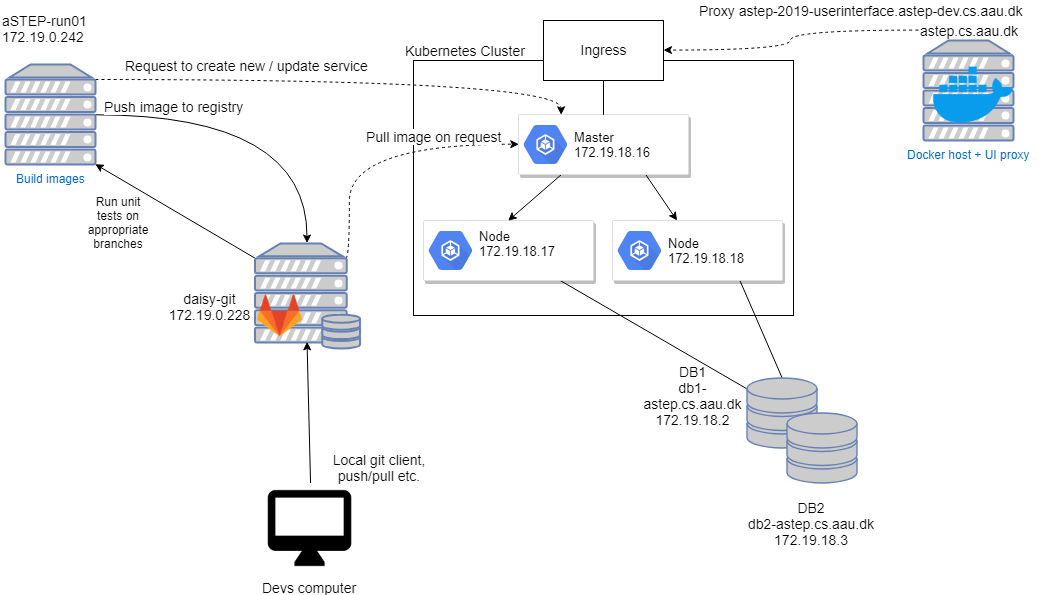
\includegraphics[width=0.9\textwidth]{Pictures/Sprint_1/server_architecture.png}
    \caption{A sketch of the server architecture of \gls{astep} \cite{astep}}
    \label{fig:server_architecture}
\end{figure}

The server architecture for \gls{astep}-2019 is robust and do not need to be changed.

\subsection{Database}
There are two different \gls{postgres} database servers (depicted as db1 and db2 in Figure \ref{fig:server_architecture}) connected to the \gls{astep} project. The databases can be used either directly with SQL queries or indirectly using a micro-service such as a \gls{graphql} service. The \gls{kubernetes} micro-service architecture has allowed each group to choose their preferred way to connect and interact with the databases. The databases and connectivity options are robust and we see no reason for them to be changed.
\section{Designing aSTEP-2020} \label{sc:tsinterface}
In section \ref{sc:astep2019}, we found that the UI, database, and server architecture are robust enough that they will need minimal or no redesigning. We also find the documentation format obscure, and in this section we propose a new format. Furthermore, we imagine that improvement could be made to the shared analytics platform.
\\\\
Our primary focus for \gls{astep}-2020 will, however, be to create an anomaly detection service for the data analytics platform.

\subsection{Documentation Service} \label{sc:docu_proposal}
We propose a new format for documentation through a new service. The format will consist of a Wiki-like service, incorporating the \gls{rfc}-list (with some changes to its purpose) as well as centralised documentation for all of \gls{astep}. Furthermore, we propose a change to the documentation shown directly in the interface.

\subsubsection{\gls{rfc}}
The \gls{rfc}-list will be moved to a Wiki-like service, and continue with some changes. Its focus will no longer be to provide documentation for the current implementation but instead will function as historical documentation of proposed changes to \gls{astep}, whether accepted or not. Each \gls{rfc} facilitates a timestamp for the proposal's creation, acceptance or rejection, and the last modification. Furthermore, each \gls{rfc} has a status (accepted/pending/rejected), and if rejected, the reasoning for rejection is described. The new \gls{rfc} list will help later semesters with decision making based on the history of proposals from the previous semesters.

\subsubsection{Shared Service/Guideline Documentation}
Documentation for shared services (such as the \gls{ui}, ServiceFetcher, etc.) will be moved to the Wiki-like service. This service should only contain documentation for current versions of implementation, and not serve as a historical reference.

\subsubsection{Service Documentation}
The new documentation format splits the service's documentation into "User Guide" and "Developer Documentation". The split in documentation will make it easier for an end-user to distinguish usage instructions as well as facilitate the extension of services by developers. The \gls{ui} will need to be changed slightly to facilitate this change. A Wiki page will contain developer documentation, and the individual services will display the Wiki page for the specific service.

\subsection{Shared Analytics Platform} \label{sc:sap}
Group SW606F20 proposes an addition to the \gls{ui} to facilitate inter-service communication better and shared analytics. This addition means that services must expose 2 additional \glspl{endpoint}, \textbf{/data}, \textbf{/combined}. \textbf{/data} must expose a service's output as raw data in JSON format. \textbf{/combined} will serve as a combination of \textbf{/render} and \textbf{/data}. Exposing a service's output, both as raw data and as a chart for rendering, will allow the \gls{ui} to use the output of one serving as the input to another. \textbf{/combined} will serve the purpose of both rendering the output of service, as well as using it as input to another. Figure \ref{fig:ui-addition} show a mock-up of the new interface.

\begin{figure}[htbp]
    \centering
    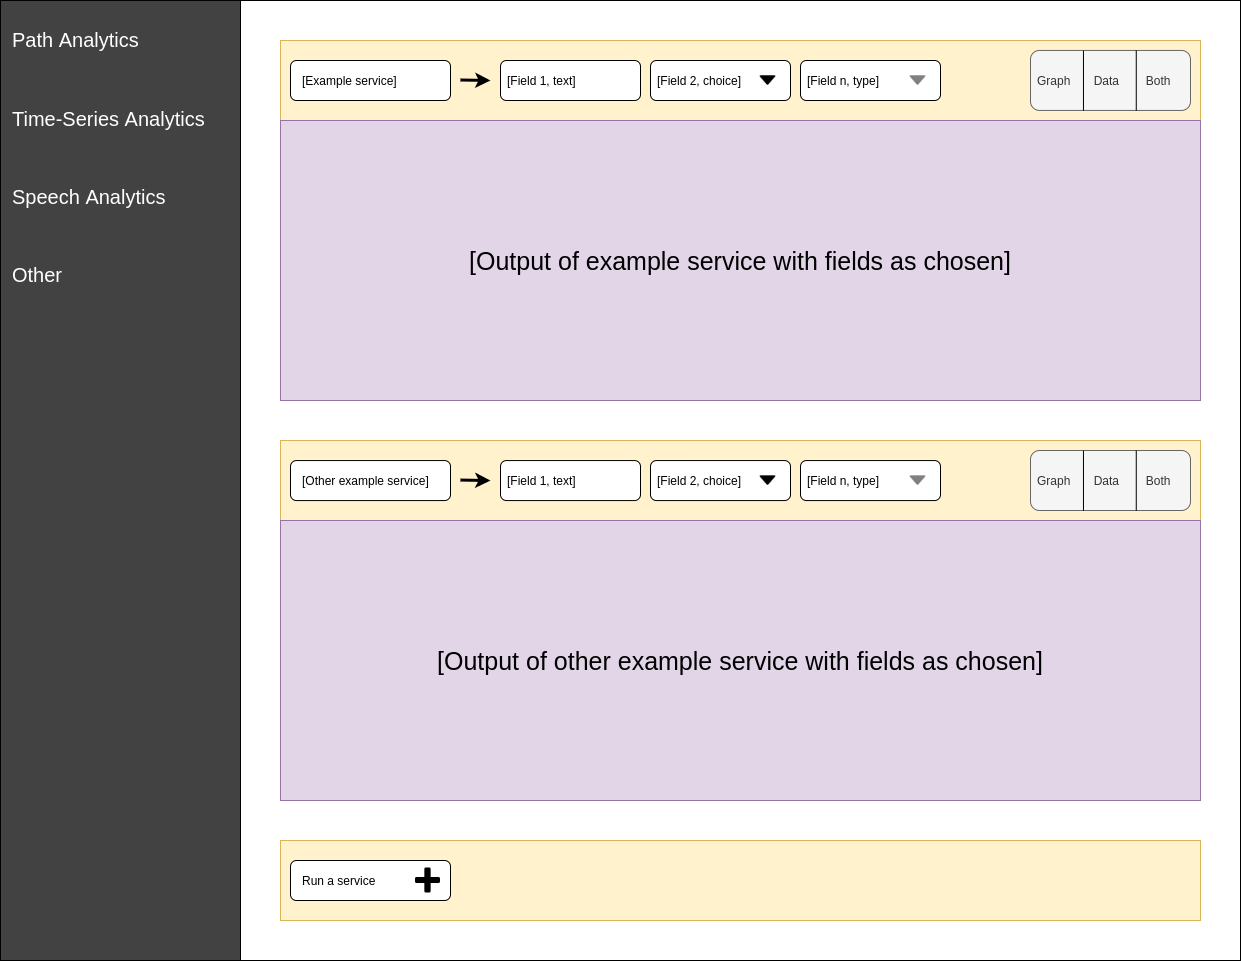
\includegraphics[width=0.8\textwidth]{Pictures/Sprint_1/single-interface.png}
    \caption{A mock-up of the addition to the \gls{astep} \gls{ui} made by group SW606F20.\cite{astep}}
    \label{fig:ui-addition}
\end{figure}

\subsection{Common Data Interface}
To further facilitate a shared analytics platform, group SW602F20 proposes a common data interface. This interface will allow the groups to work with the same data,  pass data from one service to another through the previously mentioned \gls{ui} addition. The data interface will allow the other groups to apply our anomaly detection solutions to their data before using it.
The time series subgroup decided a JSON-format would function as the data interface. Since the \gls{ui}, parses all data through JSON. Listing \ref{lst:common_interface} shows the interface.

\begin{listing}[htbp]
\begin{minted}[frame=single,
               framesep=3mm,
               linenos=true,
               xleftmargin=21pt,
               fontsize=\footnotesize,
               tabsize=4]{js}
{
  "dataSetName": "Name of dataset",
  "graphs": [
    {
      "label": "Name of graph",
      "data": [
        {
          "x": 2,
          "y": 35
        },
        {
          "x": 3,
          "y": 38
        }
      ]
    },
    {
      "label": "Name of graph",
      "data": [
        {
          "x": 5,
          "y": 33
        },
        {
          "x": 42,
          "y": 83
        },
        {
          "x": 56,
          "y": 153
        }
      ]
    }
  ]
}
\end{minted}
\caption{JSON for the common time series interface.} 
\label{lst:common_interface}
\end{listing}

The common data interface consists of several graphs, each with a label and some data points. Each data point must include an x-value and a y-value but may also include other data, such as a label for whether the point is an anomaly or not.
\section{Risk Management}
In this section, we present a risk management strategy. Risks will be identified and evaluated for comparison. For each risk, we provide a risk management strategy. We provide individual management strategies in a \Gls{rmmm}. Appendix \ref{app:B} contains the \Gls{rmmm}.

\subsection{Risk Identification}
We identify risks in two categories relevant to our project. The categories are product-specific risks and generic risks. Generic risks are known and predictable, given an arbitrary project. We base generic risks on some generic subcategories of risks applicable to every software project \cite[p.~747]{a_practitioners_approach}. Appendix \ref{app:A} illustrates both categories of risks we identified as an item checklist. In the following risk analysis, we evaluate each item on the list according to the likelihood of occurrence and consequence.


\subsection{Risk Analysis}
We assess the identified risks according to their probability (\textit{P}) of occurring, the loss (\textit{L}) of work hours, and the exposure (\textit{E}), i.e., the expected average loss of a risk. For a given risk \textit{r}, the risk's exposure \textit{E(r)} are calculated as a product of the risk's probability of occurring \textit{P(r)} and the loss \textit{L(r)}. We can only assess a given risk by evaluating both its probability and consequence, i.e., loss of work hours. Based on our knowledge of software engineering, we assess the probability of each risk. We measure the loss in lost work hours per group member to manage the risk's consequence. The loss and consequence of risk can also affect other factors than time. However, there exists no straight forward procedure when assessing a risk's consequences. Therefore, since this project has a hard deadline within four months, time will be our main focus of loss. 
\newline

\subsection{Risk Mitigation, Monitoring and Management Plan}
Appendix \ref{app:B} contains a prioritized list of risks and their plans for mitigation, monitoring, and management. Based on the list of risks and their exposure, we establish a cutoff. That is a level of exposure that is acceptable without any further strategy of risk management. The risks below this cutoff are not worth spending more time on, compared to spending the effort elsewhere. For risks above the cutoff line, we develop mitigation, monitoring, and management plans\newline 
In order to mitigate each risk, we consider risk avoidance and risk minimization. How we can reduce a risk's probability and impact should it occur, forms our mitigation plan. We also monitor each risk throughout the project. Monitoring each risk allows for management of each risk should it progress towards occurring. We finally develop a management plan for each risk, should it occur.
\section{Sprint Review} \label{sprint_1_review}
We identified the areas of \gls{astep} that should be redefined and propose changes to these. We also discussed the other groups' proposals.

Finally, we conducted a risk analysis to identify possible risks, and plan for management of these.
\noindent
\newline

\phantomsection
\newpage
\chapter{Second Sprint}

\section{Sprint Goals}
The sprint goal for the second sprint is to start designing and implementing the service. Before we design and implement our service, we analyze related work, by looking at some models used for anomaly detection. Some of these \gls{nn} models utilize methods for anomaly detection in ways irrelevant to our use case. However, analyzing these use cases help us understand the concepts and methods more in detail. After our analysis, we start the design of our service as a whole by designing the method of which to expose our service to \gls{astep}. \newline

\bgroup
\def\arraystretch{1.8}
\begin{table}[htbp]
    \centering
    \begin{tabular}{| m{7cm} |}
        \hline
        \multicolumn{1}{|>{\centering\arraybackslash}m{70mm}|}{\textbf{Goals}} \\
        \hline
        Review related work for anomaly detection. \\
        \hline
        Understand \glspl{nn} used for anomaly detection, including autoencoders,\gls{vae} and \gls{rnn}. \\
        \hline
        Design our \gls{astep} service. \\
        \hline
    \end{tabular}
    \caption{The second sprint goals.}
    \label{tab:sprint_2_goals}
\end{table}
\egroup

\noindent
Table \ref{tab:sprint_2_goals} shows a list of goals for the second sprint. The first goal is to review related work used for anomaly detection. Then we should be able to understand \glspl{nn} and their usage in anomaly detection. Understanding this will help us in the process of designing our \gls{nn} for anomaly detection. After understanding \glspl{nn}, we design the service we expose to \gls{astep}. Section \ref{sprint_2_review} evaluates these goals in the sprint review.

\section{Neural Networks}
Neural networks are computational models comprised of neurons organized in layers. An advantage of neural networks is their ability to learn. The ability to learn means neural networks can handle complex tasks such as image recognition or anomaly detection. 

\begin{figure}[htbp]
    \centering
    \includegraphics[width=0.9\textwidth]{Pictures/Sprint_2/Neuron_Structor.png}
    \caption{The structure of a neuron.}
    \label{fig:NeuronStructor}
\end{figure}
\noindent
Neurons are mathematical models based on the neurons in the brains of animals and humans. Figure \ref{fig:NeuronStructor} shows the structure of an artificial neuron. The input $x$ of a neuron is the output of neurons from the previous layer or direct values from a dataset. The output of a neuron is calculated using the inputs and weights of all the neurons in the previous layer, a bias, and an activation function, through the following equation:

\begin{equation}
    y_k = \phi(\sum_{j=1}^{n} w_{kj} x_j b)
\end{equation}

Where $y_k$ is the output of the \textit{k}th neuron, $x_j$ is output of the \textit{j}th neuron in the previous layer, $w_{kj}$ the weight between the \textit{j}th neuron in the previous layer and the \textit{k}th neuron in this layer, $b$ is the bias and $\phi$ is the activation function. Many different activation functions exist for different purposes.

Neural networks learn by training. Training of a neural network consists of giving the network of input data. For each input, the network provides an output. The training process then calculates a loss between the actual output and the expected output is given the input. Many different loss functions exist to provide different learned behavior. The training process uses the loss to update the weights between neurons in a process called backpropagation. The purpose of updating the neurons is to improve the model at its task.
\section{Related Work}\label{sec:related_work}
In this section, we explore \gls{nn} models that have use cases in anomaly detection, as well as some related work that utilizes these models for this purpose.

\subsection{Autoencoder}
An autoencoder is a type of unsupervised \gls{nn}. Figure \ref{fig:autoencoder} shows the architecture of an autoencoder.


\begin{figure}[htbp]
    \centering
    \includegraphics[width=0.85\textwidth]{Pictures/Sprint_2/autoencoder.png}
    \caption{Architecture of an autoencoder.}
    \label{fig:autoencoder}
\end{figure}

\noindent
The purpose of an autoencoder is to learn a representation of given input data. Autoencoders achieve this by learning to compress and encode the input data, and from this encoded version of the input, reconstruct the data using a decoder. An autoencoder consists of at least three main parts: An encoder, a decoder, and a bottleneck. The encoder consists of a \gls{visiblelayer} and some \glspl{hiddenlayer}. Layer $i$ in the encoder has the same or fewer neurons than layer $i-1$. Decreasing the number of neurons in the inner layers compress and encodes the input data. The last \gls{hiddenlayer} of the encoder (the middle layer) is also the input layer for the decoder. The decoder consists of the input layer and some additional \glspl{hiddenlayer}, with an output layer at the end (\gls{visiblelayer}). The decoder's job is the opposite of the encoder. The decoder gets the output of the encoder and decodes it to reconstruct the original data. Together the encoder and decoder create a bottleneck, also called the latent vector representation or code layer, as seen in Figure \ref{fig:autoencoder}. \Gls{backprop} using \gls{graddesc} is used during the training to reduce reconstruction loss by changing weights and biases in the neurons \cite{autoencoder_used}\cite{autoencoder_into}. The loss function usually used in autoencoders is mean squared error:\newline
\begin{equation}
    J(x, z)=\lvert x - z \rvert^2
\end{equation}
Where $x$ is the original input and $z$ is the reconstructed input.

In \cite{hawkins_he_williams_baxter_2002} anomaly detection is performed on large multivariate databases through the use of a Replicator Neural Network (of which autoencoders are a subcategory). The Replicator Neural Network attempts to replicate each input data point. The average reconstruction error over all variables determines the outlier factor. A higher outlier factor means a higher likelihood that the data point is an outlier. This method proves useful in determining outliers, effectively identifying intrusions in a network intrusion data set, as well as correctly identifying 77\% of cases in a breast cancer data set.

\subsection{Variational Autoencoder}\label{sc:vae}
A \gls{vae} is a stochastic \gls{nn} and generative model, based on autoencoders. Generative models all share the feature of generating new data based on existing data. The decoder network of an autoencoder can be considered a generative model since it generates new data based on the latent vector provided by the encoder network. However, the encoder network determines the latent vector based on the original input. Thus, to generate new data, the latent vector must contain data that is not a direct encoding of input data.
In theory, it is possible to randomly inject some data into the latent vector, and have the decoder network generate some data based on the injected data. However, since the latent vector is inherently latent, we cannot assume that injected data has any meaning to the decoder. Given an autoencoder network trained to reconstruct images, randomly assigning a latent vector will probably result in images that are just noise.

\Glspl{vae} attempt to solve this problem. In a \gls{vae}, the latent vector represents a probability distribution instead of real values. The latent vector is two vectors, a mean vector, and a standard deviation vector. Figure \ref{fig:architecture_vae} shows the architecture of a \gls{vae}. The figure also shows how two vectors form the latent vector, and the decoder samples from these vectors to obtain input.

\begin{figure}[htbp]
    \centering
    \includegraphics[width=0.85\textwidth]{Pictures/Sprint_2/vae.png}
    \caption{The architecture of a \gls{vae}. $\boldsymbol{\mu}$ is the mean vector and $\boldsymbol{\Sigma}$ is the standard deviation vector.}
    \label{fig:architecture_vae}
\end{figure}

Training the encoder network can allow it to capture the probability distribution of the input data set. The decoder network can sample from the distribution and generate a new output that follows the same probability distribution and thus resembles the input data set, while at the same time being new data. The sampling of the distribution, however, present some new problems.

Firstly, the \gls{lossfunc} needs to be changed, since training the \gls{vae} based on the Euclidean Distance and Sigmoid Cross Entropy function alone, will result in probability distributions that essentially "hard-code" the inputs as distributions. We want to force the network to generate probability distributions that follow a Gaussian distribution, such that the network will focus on features shared between the inputs instead of just encoding the specific input. To enforce this, we introduce a composite cost function, consisting of both the original Euclidean Distance and Sigmoid Cross Entropy functions, and the \gls{kldiv}. \gls{kldiv} measures how much one distribution is different from another. Using this, we can penalize the network for generating distributions that are far from a Gaussian distribution \cite{understanding_vae}.

Secondly, we run into a problem when attempting \gls{backprop} on this network, since a sample of a probability distribution cannot be differentiated (as required by \gls{backprop} with \gls{graddesc}). To solve this problem \glspl{vae} utilize the reparameterization-technique. The technique performs sampling from a unit Gaussian distribution (a Gaussian distribution with mean 0 and standard deviation 1) and then computes the sample vector $z$ by:
\begin{center}
\begin{equation}
    z = \boldsymbol{\mu}(X) + \boldsymbol{\sigma}^{1/2}(X) * \epsilon
    \label{eq:reparameterization}
\end{equation}
\end{center}
Where $\boldsymbol{\mu}(X)$ is the mean vector, $\boldsymbol{\sigma(X)}$ is the standard deviation vector, and $\boldsymbol{\epsilon}$ is a vector of samples of a unit Gaussian distribution, given by $\epsilon \sim \mathcal{N}(0,1)$. 
The reparameterization-technique moves the sampling operation away from the mean and standard deviation vectors, which need to be differentiable for stochastic \gls{graddesc}, thus allowing for \gls{backprop} \cite{doersch2016tutorial}. Figure \ref{fig:vae:reparam} shows the reparameterization technique on a \gls{vae} architecture.

\begin{figure}[htbp]
    \centering
    \begin{subfigure}{0.5\textwidth}
    \centering
    \includegraphics[width=0.9\linewidth]{Pictures/Sprint_2/ReparameterizationTechniqueWithout.png}
    \caption*{\gls{vae} without reparameterization technique}
    \end{subfigure}%
    \begin{subfigure}{0.5\textwidth}
    \centering
    \includegraphics[width=0.8\linewidth]{Pictures/Sprint_2/ReparameterizationTechniqueWith.png}
    \caption*{\gls{vae} with reparameterization technique.}
    \end{subfigure}%
\caption{VAE with and without the reparameterization technique. Red indicates sampling operations which are non-differentiable. Blue indicates loss functions.}\label{fig:vae:reparam}
\end{figure}

\cite{vae_anomaly_detection} shows the use of a \gls{vae} for anomaly detection in seasonal key performance indicators for a top internet company. The technique shows excellent performance, with \gls{f1score} ranging from 0.7 to 0.9.

\cite{hawkins_he_williams_baxter_2002} and \cite{vae_anomaly_detection} shows that autoencoders and \glspl{vae} perform well for anomaly detection. However, these network types are not able to perform analysis on sequential data, such as time series data (\cite{vae_anomaly_detection} perform analysis on time series data, but uses a sliding window algorithm to make it non-sequential). The inability to handle sequential data means that these networks cannot capture the temporal dependencies of sequential data, and therefore are not suitable for time series anomaly detection.

\subsection{Recurrent Neural Network}
A \gls{rnn} is a type of \gls{nn} used for sequential data. In a standard feed-forward \gls{nn}, output, weights, and biases are based solely on input. Standard feed-forward \gls{nn} treats all inputs and outputs independently. When working with sequential data, this is no longer the case. For example, if we want to create a \gls{nn} for translating natural language sentences, a correct translation cannot necessarily be achieved by merely translating each word, one after the other since words in a sentence can have meanings that depend on the other words in the sentence.\cite{rnn_tutorial}

A \gls{rnn} computes output that is dependant on, the input and previous inputs. A \gls{rnn} consists of 3 parts: an input $\boldsymbol{x}$, an output $\boldsymbol{o}$ and a hidden state $s$ (similar to the \glspl{hiddenlayer} of standard \glspl{nn} and autoencoders). These are all parts that also exist in standard \glspl{nn} however a \gls{rnn} calculate them differently. A \gls{rnn} does the same computation repeatedly for each input in a sequence while retaining some information in the hidden state. If we "unfold" a \gls{rnn} by putting the network for each input beside each other it looks like Figure \ref{fig:unfolded_rnn}.\cite{rnn_tutorial}

\begin{figure}[htbp]
    \centering
    \includegraphics[width=0.85\textwidth]{Pictures/Sprint_2/rnn_unfolded.png}
    \caption{An unfolded \gls{rnn}. $\boldsymbol{x}$ is input, $\boldsymbol{o}$ is output, and $s$ is hidden state. Subscripts indicate time series steps.\cite{rnn_tutorial}}
    \label{fig:unfolded_rnn}
\end{figure}

If we study figure \ref{fig:unfolded_rnn}, we can see that for a time series step $t$, output $\boldsymbol{o_t}$ depends on the \gls{hiddenlayer} $s_t$, which depends on not only the input $\boldsymbol{x_t}$, but also the hidden state for the previous time series step $s_{t-1}$. This allows the network to retain some information between inputs.\cite{rnn_tutorial}

As with other \gls{nn} extensions, \glspl{rnn} presents some problems that need to be addressed. Most significantly, \glspl{rnn} have a problem known as vanishing gradient problem.\cite{rnn_tutorial}

When training a \gls{rnn}, using \gls{backprop}, the network shares parameters between all time steps. At each time step, the gradient depends not only on the current time step but also the previous time steps. This dependency means that the model has to backpropagate gradients throughout the time steps. Due to the nature of \gls{backprop}, this means that \glspl{rnn} have difficulties with learning long-term dependencies, i.e., dependencies between steps that are further apart.\cite{rnn_tutorial}

Variations of \glspl{rnn} exist that counteract the vanishing gradient problem, such as \gls{lstm} and \gls{gru}. \gls{lstm} networks contain units with three gates: input gates, forget gates, and output gates. The forget gate defines how much the unit should remember from the previous hidden state. The input gate determines how much of the newly computed state should determine the new hidden state. The output gate determines how much of the new hidden state the unit exposes to the rest of the network.\cite{lstm_gru_tutorial}

\gls{gru} and \gls{lstm} both use gates that define how they compute the hidden state. However, \gls{gru} only contains two gates: reset gates and update gates. Reset gates determine how the previous hidden state should combine with the current input. The update gate determines what the neural unit remembers of the previous hidden state.\cite{lstm_gru_tutorial}

\cite{related_work_rnn} shows the use of an LSTM-network for use in multivariate time series prediction, and uses prediction errors to determine anomalies.

\subsection{Variational Autoencoder With Recurrent Layers}
A \gls{vae} with recurrent layers is a type of \gls{vae}, where some of the dense layers are replaced by a \gls{rnn}, such as \gls{lstm} or \gls{gru}. Such a network can achieve a "best-of-both-worlds" result, where the \gls{rnn} layers are used to capture the temporal dependencies that are inherent with time-series data, while the \gls{vae} can elicit the stochasticity that is also present in time series data.

\cite{kdd} use a \gls{vae} with \gls{rnn} layers approach for anomaly detection on multi-variate time series data. They use a combination of \gls{gru} cells, and a \gls{vae} to attempt to reconstruct each data point based on previous data points and determine for each reconstructed data point, how accurate the model was able to reconstruct it, compared to the actual data point. From this, they can compute a reconstruction probability, and if that probability is lower than a threshold, which they compute via Extreme-Value Theory, the point is labeled as an anomaly. They were able to achieve great results with this approach, with an overall F1-score of 0.86.
\input{Report/Sprint_2/common_interface}
\section{aSTEP Service Design}\label{sec:service_design}
In this section, we design our service for implementation on \gls{astep}-2020. The neural network model is only part of the service as a whole.
Figure \ref{fig:service-component} shows the architectural design of the entire service. Implementing the necessary \glspl{endpoint} to allow our service to be shown in the \gls{ui} is desired, as this \gls{ui} will allow more inexperienced users access to the service. Figure \ref{fig:service-component} displays the necessary interfaces that the service must implement to be shown in the \gls{astep} \gls{ui}. This implies an interface to receive input from other services and an interface for output from the service to other services.

\begin{figure}[htbp]
    \centering
    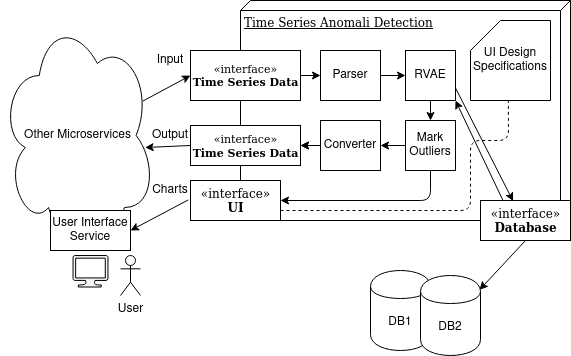
\includegraphics[width=0.85\textwidth]{Pictures/Sprint_2/ComponentArchitecture.png}
    \caption{Architecture of the service.}
    \label{fig:service-component}
\end{figure}

\subsection{Interfaces}
The interfaces to our application are:
\begin{itemize}
    \item Time Series Data
    \item UI
\end{itemize}
The interfaces are all marked in the component design figure \ref{fig:service-component} as interfaces.
The Time Series Data and \gls{ui} interfaces have been designed in collaboration with other groups and thus we have little say in how these interfaces work.

\subsection*{Time Series Data}
For the Time Series Data interface we follow the standard proposed by SW602F20, discussed in Section \ref{sc:tsinterface}. 

In the addition made to the \gls{ui}, discussed in Section \ref{sc:sap}, it was also decided that services should specify, at the \textbf{/info} \gls{endpoint}, the type of data that is expected as input, and the type of data that will be returned as output (at \textbf{/data}, \textbf{/combined}, \textbf{/render}). For the Time Series Interface, the name \textit{time-series} was chosen. The fields that are added at the \textbf{/info} \gls{endpoint} can be seen in Listing \ref{lst:info_added_fields}.

\begin{listing}[htbp]
    \begin{minted}[breaklines, linenos, escapeinside=||]{javascript}
    "input": [ {
        "name": "data-input",
        "label": "Input data",
        "type": "time-series"
    } ],
    "output": [ {
        "name": "data-output",
        "label": "Output data",
        "type": "time-series"
    } ]
    \end{minted}
    \caption{The time series interface is specified by setting it as input type.}
    \label{lst:info_added_fields}
\end{listing}

\subsubsection*{UI}
For the \gls{ui}, we must adhere to a standard, set forth by the \gls{astep}-2020 committee, that specifies some endpoints that we must expose with some specific data. In return our service will be visible within the \gls{astep} \gls{ui}.

The required endpoints are:
\begin{itemize}
    \item /info
    \item /readme
    \item /fields
    \item /render
    \item /data
    \item /combined
\end{itemize}
These endpoints must be exposed to the \gls{astep} \gls{ui} using a web server.
\section{Sprint Review} \label{sprint_2_review}
We have reviewed and explored multiple types of related work within anomaly detection. This includes multiple types of \glspl{nn} such as \gls{vae} and \gls{rnn}. By exploring this related work, we intuitively and theoretically got an understanding of \glspl{nn} and their use cases within anomaly detection. We discovered that both \gls{vae} and \gls{rnn} by themselves are not suitable for anomaly detection on time series data, however a combination of the two, \gls{rvae}, has seen use with great results.

Furthermore, our service component architecture was designed and the required interfaces and corresponding \glspl{endpoint} were explained.

\phantomsection
\newpage
\chapter{Third Sprint}
\section{Sprint Goals}
The sprint goals for the third sprint are to continue designing and implementation of the service. The first goal is to design the architecture of the \gls{nn}, so we can then implement it. Before the implementation of the model, we also explore different technology available to do so. We need a machine learning framework and a web framework. We implement the \gls{nn} trained on univariate and multivariate data. After training and ensuring the model works correctly, we expose the service to \gls{astep}.\newline

\bgroup
\def\arraystretch{1.8}
\begin{table}[htbp]
    \centering
    \begin{tabular}{| m{7cm} |}
        \hline
        \multicolumn{1}{|>{\centering\arraybackslash}m{70mm}|}{\textbf{Goals}} \\
        \hline
        Design the \gls{nn} architecture. \\
        \hline
        Assess relevant implementation technology. \\
        \hline
        Implement and train the \gls{nn}. \\
        \hline
        Expose the \gls{nn} to \gls{astep}. \\
        \hline
    \end{tabular}
    \caption{The third sprint goals.}
    \label{tab:sprint_3_goals}
\end{table}
\egroup

\noindent
Table \ref{tab:sprint_3_goals} shows a list of goals for the third sprint. The first goal is to design the \gls{nn} architecture. The second goal is to explore and assess relevant technology for implementation. The third goal is to implement the \gls{nn}. As our fourth goal, we should be able to expose the service to \gls{astep} so that others can use the service. Section \ref{sprint_3_review} evaluates these goals in the sprint review.

\section{Network Architecture}
In this section we design the architecture of our \gls{nn}. In section \ref{sec:related_work}, we explored \gls{nn} models that have applications in anomaly detection, as well as some related work that utilize these models for anomaly detection. Based on the findings in that section, we decide to base our \gls{nn} on the findings of \cite{kdd}, and construct a \gls{vae} with \gls{rnn} layers.

\subsection{Overall Structure}
We design a model for anomaly detection on multivariate time series data. It detects anomalies at the \gls{entity_level}, which means that it does not consider each univariate time series when determining whether an input is anomalous, but rather all the time series in a union.

Our model overall consists of two parts: a training module and a prediction module. Furthermore, we carry out some preprocessing of data as well as some postprocessing of results. Figure \ref{fig:nn_struct} shows the overall structure of our model.

\begin{figure}[htbp]
    \centering
    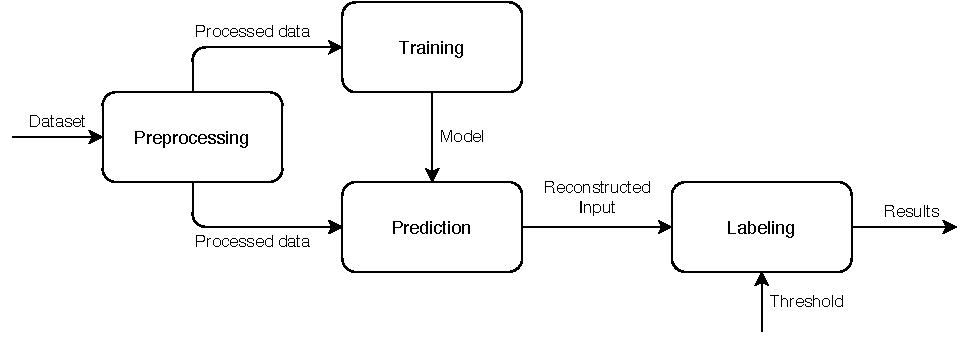
\includegraphics[width=0.9\textwidth]{Pictures/Sprint_3/NetworkStructure.pdf}
    \caption{The overall structure of our \gls{nn} model.}
    \label{fig:nn_struct}
\end{figure}
\noindent
We first perform preprocessing of the input dataset. Preprocessing is done by normalizing the input between 0 and 1, then dividing inputs into \gls{slwi} of some given size. This is done to allow the \gls{rnn} layers to capture temporal dependencies.
\\\\
The processed dataset is passed to the training module to train the model. The model is taught to reconstruct the input data as a probability distribution, such that it captures the standard patterns present in the exact data. This will, in turn, enable us to use reconstruction probabilities to determine whether a data point is anomalous.
\\\\
When the model has been trained, it may be stored and used for prediction on datasets with similar patterns. When predicting, the model will output a reconstruction of the input. This is used to compute labels for each input point.                            
\\\\
Labeling consists of computing the reconstruction probability of each input, and if that probability is lower than a threshold, the model label the input as anomalous.

\subsection{Model Architecture}
As previously explained, the model is based on the \gls{vae} model, with elements of \gls{rnn} networks, more specifically we choose to use \gls{gru} as the recurrent element in our model.

The architecture is divided into 2 logical parts, the encoder network and the decoder network. These 2 parts are very similar to the encoder and decoder networks found in auto-encoders and \glspl{vae}. Figure \ref{fig:nn_arch} shows the architecture of the encoder network and decoder network, side-by-side.

\begin{figure}[htbp]
    \centering
    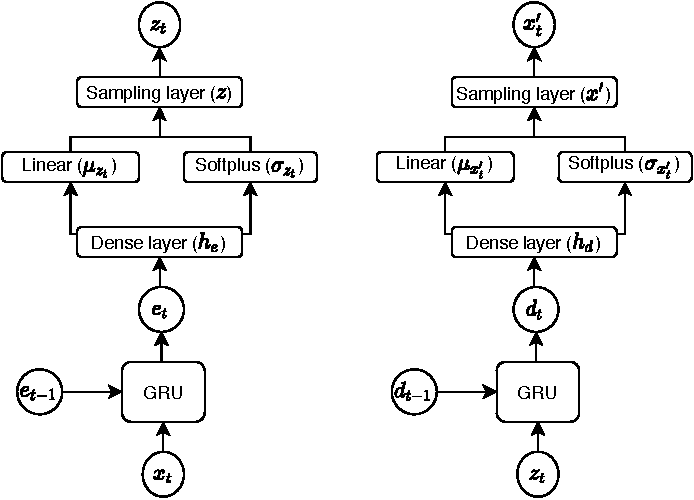
\includegraphics[width=0.8\textwidth]{Pictures/Sprint_3/NetworkArchitecture.pdf}
    \caption{Architecture of the \gls{nn}. On the left is the encoder and on the right is the decoder.}
    \label{fig:nn_arch}
\end{figure}

The encoder network consists of a \gls{gru} layer, which at time $t$ receives input $x_t$ and previous hidden state of the \gls{gru} $e_{t-1}$ to generate the hidden state $e_t$. Then $e_t$ is sent to a dense layer, $h_e$, to generate mean and standard deviation for $z_t$, $\mu_{z_t}$ and $\sigma_{z_t}$. Sampling is performed on these, as per a standard \gls{vae} through the reparameterization technique, to obtain $z_t$.

The decoder network is largely the same as the encoder network. The \gls{gru} layer receives a latent space variable at time t, $z_t$, and hidden state from previous timestep, $d_{t-1}$. The hidden state in the encoder network $e_t$ is not the same as in the decoder network $d_t$. The \gls{gru} layer then outputs hidden state $d_t$ and this is sent to the decoders dense layer, $h_d$, which in turn outputs the mean and standard deviation of $x'$, $\mu_{x'_t}$ and $\sigma_{x'_t}$.

The whole model's output is $x'_t$, which is a reconstruction of input $x$ at timestep $t$.

\subsection{Model Training}
he model can be trained by using Stochastic \gls{graddesc}.
The loss function consists of the negative reconstruction error (or negative log-likelihood) combined with the \gls{kldiv}. Thus when optimizing, we are training the network to properly reconstruct inputs based on the latent z-space variables, as well as training the network to encode inputs into a normally distributed probability distribution properly.

\subsection{Detection}
Determining whether an input $x_t$ is anomalous, the reconstruction probability of the input is calculated. The reconstruction probability of an input is a number describing how likely an input is based on the encoded latent space variable.
\\\\
Reconstruction probability $S$ is given as the following:

\begin{equation}
    S = log(p_\Theta(x_t | z_{t}))
\end{equation}

\noindent
Which is the log-probability of $x_t$ given $z_t$ and $\Theta$, where $\Theta$ are the parameters of the decoder network. If we think of the decoder network is a deterministic function that maps $z_t$ to $x'_t$, we get:

\begin{equation}
    S = log(p(x_t | x'_t))
\end{equation}

\noindent
If we assume that the $p(x_t | x'_t)$ distribution has a Gaussian form, which it should, given the applied \gls{kldiv} we get:

\begin{equation}
    S = log(p(x_t | x'_t)) \sim log e^{|x-x'|^2} \sim (x - x')^2
\end{equation}

\noindent
The decoder network is, however, not a deterministic function, but rather a stochastic function, because of the sampling layer. This means that to accurately use $(x - x')^2$, firstly, $z_t$ should be sampled many times from $\mu_{z_t}$ and $\sigma_{z_t}$, the mean of these samples calculated, and this be used as the input to the decoder network. $x'_t$ should likewise be sampled many times from $\mu_{x'_t}$ and $\sigma_{x'_t}$ and the mean should be used as $x'_t$.
\\\\
After the reconstruction probability is calculated for a single input, we need to compare it to the rest of the inputs, to determine the anomalies. This is done by computing a z-score (or standard score) for each reconstruction probability, based on all the reconstruction probabilities. The formula for calculating an inputs z-score is given as:

\begin{equation}
    \text{z-score} = \frac{x - \mu}{\sigma} 
\end{equation}

\noindent
Where $x$ is the input, $\mu$ is the mean of all the reconstruction probabilities, and $\sigma$ is the standard deviation of all the reconstruction probabilities.
\\\\
When the labeling module has calculated z-scores, it compares the scores to a threshold. A threshold is selected based on the percentile of anomalies in the input dataset. The module will label the percentile worst reconstruction probabilities as anomalies. 
For example, if a dataset is known to have $\approx 5\%$ anomalies, $\approx 2$ should be selected as a threshold, and this will mean that the $\approx 5\%$ inputs with the worst reconstruction probabilities will be labeled as anomalies.
\section{Technology Assessment} \label{sc:technology_assessment}
In this section, we explore the technologies available for both machine learning and serving web pages.

\subsection{Machine Learning Framework}
We use a framework instead of implementing the \gls{nn} from scratch, as it will save us time, and abstract away details. The implementation details of the network will depend on which framework we choose, as not all frameworks provide the same level of abstraction.

The \gls{astep} server uses a \gls{kubernetes} cluster to handle the services, and as such, the language and framework can be any that can run in a docker container. Containers increase the options, but we will only explore a small subset of possible combinations.

\subsubsection*{TensorFlow}
\gls{tensorflow} is an open-source platform for machine learning developed by Google, who uses it for research and production of machine learning applications \cite{GoogleTensorflowOpenSourced}. \Gls{tensorflow} allows researchers to abstract away lower-level software engineering and focus on their models. A comprehensive set of tools and libraries enable \gls{tensorflow} to obtain this abstraction \cite{TensorFlow}. 

One of the tools \gls{tensorflow} supports to abstract away details is \gls{keras}. \Gls{keras} is an open-source API capable of running on top of \gls{tensorflow}. By being modular, composable, and extendable, \gls{keras} supports abstraction away from low-level software engineering concerns. A \gls{keras} model is composed of modules such as layers. Researchers and developers can make custom modules and thereby extend \gls{keras} to support new ideas \cite{Keras}.

\subsubsection*{PyTorch}
\Gls{pytorch} is an open-source python wrapper for Torch, a scientific computing framework, developed by Facebook AI research team. \Gls{pytorch} provides GPU-acceleration for the training of neural networks and multi-processing with shared memory. \gls{pytorch} can also be used to complement or replace functions in existing packages such as NumPy by providing GPU-acceleration for tensor computation \cite{PyTorch2}.

\subsubsection*{Deeplearning4j}
\gls{dl4j} is an open-source machine learning framework for the JVM \cite{dl4j}. Since \gls{dl4j} is for the JVM, it can use Java, Scala, Clojure, and Kotlin, while \gls{tensorflow} and \gls{pytorch} are mainly focused on Python. \gls{dl4j} supports distributing training workloads over multiple clients with Hadoop and Spark.

\subsubsection*{Subconclusion}
We choose to use \gls{tensorflow} as our machine learning framework, since \gls{tensorflow} is a framework that we have worked with in previous projects, and the extra features from other frameworks are not needed. Furthermore, to abstract away low-level software engineering concerns, \gls{tensorflow} supports \gls{keras}. \gls{keras} allows us to entirely focus on the model, without concern about minor technicalities. We assess that the combination of \gls{tensorflow} and \gls{keras} fits our purpose of using the best.

\subsection{Web Framework}
We will use the web framework to implement the \glspl{endpoint} for the interfaces we chose in the design section, advanced features and scalability is not needed.
\subsubsection*{Flask}
Flask is a microframework for web applications. Flask focuses on a simple core structure but still supports extensions. Extensions enable Flask to handle database integration, form validation, upload handling,  authentication, and more. The simple core structure and extendability make Flask able to accommodate many different preferences and requirements. The core of Flask depends on a few libraries, mainly Werkzeug to implement WSGI and Jinja2 to handle templating \cite{DesignFlask, DependenciesFlask}.

\subsubsection*{Django}
Django is a high-level web framework. Django focuses on fast development, security, and scalability. Django takes care of a lot of the work from web development to give faster development and security, by having security included in functions to avoid common security mistakes. Django also includes features like user authentication, content administration, site maps, RSS feeds.

\subsubsection*{Subconclusion}
As we only need the ability to expose the service to some endpoints, the extra features included in Django are not needed. We also have previous experience working with Flask. We will, therefore, use Flask as a framework to incorporate the \gls{nn} into \gls{astep}.
\section{Network Implementation}
In this section we describe the implementation of the \gls{nn}.

We start the implementation of the \gls{nn} by developing the preprocessing needed to use the data for training and predicting. The model is designed to work on multivariate data, but to make sure the architecture and model works, we first train it on univariate data.



\subsection{Data Preprocessing}
The data preprocessing is the first stage of the network. Both the training and prediction modules use the preprocessing module on the input before training or predicting data. To load the data and transform it into an object \gls{tensorflow} can use, we create a dataset class. The Dataset class can load data from CSV files and \gls{tensorflow} datasets, and transform the data to several other outputs, like \gls{tensorflow} dataset, matplotlib plots, and to charts used for the time series interface on \gls{astep}. Listing \ref{lst:to_tf_dataset} shows how the data is transformed to a \gls{tensorflow} dataset. When the data is transformed into a \gls{tensorflow} dataset, we normalize the data and apply \gls{slwi}. We normalize the data, and we apply \gls{slwi} to segment the data into sequences. Listing \ref{lst:normalize} shows how the normalization is done, and Listing \ref{lst:make_windows} shows how \gls{slwi} is applied.

\begin{listing}[htbp]
\begin{minted}
[
frame=single,
framesep=3mm,
breaklines,
linenos=true,
xleftmargin=21pt,
fontsize=\footnotesize,
tabsize=4
]
{Python}
def to_tf_dataset(self, window_size, batch_size):
    rv = np.zeros(shape=(len(self.graphs[0].data), len(self.graphs)))
    for i, graph in enumerate(self.graphs):
        for j, data_point in enumerate(graph.data):
            rv[j][i] = data_point.y
    rv = normalize(rv)
    rv = make_windows(rv, window_size)
    rv = tf.data.Dataset.from_tensor_slices((rv, rv))
    rv = rv.batch(batch_size, drop_remainder=False)
    return rv
\end{minted}
\caption{\texttt{to\_tf\_dataset} function in \texttt{Dataset} class.}
\label{lst:to_tf_dataset}
\end{listing}

\noindent

\begin{listing}[htbp]
\begin{minted}
[
frame=single,
framesep=3mm,
breaklines,
linenos=true,
xleftmargin=21pt,
fontsize=\footnotesize,
tabsize=4
]
{Python}
def normalize(data):
    max_d = max(max(data, key=lambda x: max(x)))
    min_d = min(min(data, key=lambda x: min(x)))

    # We dont wanna divide by zero when min == max
    if max(data) == min(data):
        return [[0 for y in x] for x in data]
    return [[(y - min_d) / (max_d - min_d) for y in x] for x in data]
\end{minted}
\caption{\texttt{normalize} function in \texttt{preprocessing.py}}
\label{lst:normalize}
\end{listing}

\noindent

\begin{listing}[htbp]
\begin{minted}
[
frame=single,
framesep=3mm,
breaklines,
linenos=true,
xleftmargin=21pt,
fontsize=\footnotesize,
tabsize=4
]
{Python}
def make_windows(data, length=1):
    # Window cannot be bigger than input size
    if length > len(data):
        length = len(data) - 1

    windows = []
    for i in range(len(data) - length + 1):
        windows.append(data[i:i + length])
    return windows
\end{minted}
\caption{\texttt{make\_windows} function in \texttt{preprocessing.py}.}
\label{lst:make_windows}
\end{listing}

\noindent


\subsection{Implementation of The Network}
We implement the network in \gls{tensorflow} using \gls{keras}. The first part of implementing the network is to define the sizes of the layers and the input shape. As we want the same dimensions for both the encoder and the decoder, this makes it easier to change the dimensions of the GRU and dense layers. Listing \ref{lst:network_parameters} shows the parameters of the network, including sizes of the layers and window size. These parameters will be tuned in future testing to find optimal values.

\begin{listing}[htbp]
\begin{minted}
[
frame=single,
framesep=3mm,
breaklines,
linenos=true,
xleftmargin=21pt,
fontsize=\footnotesize,
tabsize=4
]
{Python}
batch_size = 32
window_size = 64
features = 1
gru_dim = 32
dense_dim = 32
\end{minted}
\caption{Network parameters.}
\label{lst:network_parameters}
\end{listing}

\noindent
The second part of implementing the network is to implement the encoder. The input layer is the first layer of the encoder. Which is the layer all the windows will be fed to, in order to get the right shape for the input to the GRU layer. When the input layer is defined, we feed the input through the rest of the encoder. Listing \ref{lst:encoder} shows the implementation of the encoder.

\begin{listing}[htbp]
\begin{minted}
[
frame=single,
framesep=3mm,
breaklines,
linenos=true,
xleftmargin=21pt,
fontsize=\footnotesize,
tabsize=4
]
{Python}
def make_encoder(batch_size, window_size, features, gru_dim, dense_dim):
    input = keras.Input(shape=(window_size, features), name='encoder_input')
    gru = keras.layers.GRU(gru_dim, return_sequences=True, name='encoder_gru')(input)
    dense = keras.layers.Dense(dense_dim, name='encoder_dense', activation='relu')(gru)
    z_mean = keras.layers.Dense(features, name='encoder_z_mean', activation='linear')(dense)
    z_log_var = keras.layers.Dense(features, name='encoder_z_log_var', activation='softplus')(dense)
    z_mean, z_log_var = KLDivergenceLayer()([z_mean, z_log_var])
    z_sample = keras.layers.Lambda(sampling, name='encoder_z_sample',
                                   output_shape=(None, window_size, features))([z_mean, z_log_var])

    encoder = keras.Model(input, z_sample, name='encoder')
    return encoder, input
\end{minted}
\caption{Encoder.}
\label{lst:encoder}
\end{listing}

\noindent
After the input layer, the data is fed through the GRU and Dense layers. After the dense layer, are the \texttt{z\_mean} and \texttt{z\_log\_var} latent vectors, implemented as dense layers. The \texttt{z\_mean} and \texttt{z\_log\_var} is the input to a \gls{kldiv} layer. The \gls{kldiv} layer is a passthrough layer that simply outputs its input, but adds a loss to the model, computed as the \gls{kldiv} between the distribution formed by the \texttt{z\_mean} and \texttt{z\_log\_var} latent vectors and a unit Gaussian distribution. Refer to equation X. Listing \ref{lst:kld_layer} shows the implementation of our \gls{kldiv} layer.

\begin{listing}[htbp]
\begin{minted}
[
frame=single,
framesep=3mm,
breaklines,
linenos=true,
xleftmargin=21pt,
fontsize=\footnotesize,
tabsize=4
]
{Python}
class KLDivergenceLayer(keras.layers.Layer):
    def __init__(self, *args, **kwargs):
        self.is_placeholder = True
        super(KLDivergenceLayer, self).__init__(*args, **kwargs)

    def call(self, inputs, **kwargs):
        mu, log_var = inputs

        kl_batch = - .5 * keras.backend.sum(1 + log_var -
                                            keras.backend.square(mu) -
                                            keras.backend.exp(log_var), axis=-1)

        self.add_loss(keras.backend.mean(kl_batch), inputs=inputs)

        return inputs
\end{minted}
\caption{\gls{kldiv} Layer class.}
\label{lst:kld_layer}
\end{listing}

\noindent
The the \texttt{z\_mean} and \texttt{z\_log\_var} returned from the \gls{kldiv} layer are then used to sample. This is done using the \texttt{Lambda} layer from \gls{keras}, which applies the sampling function the inputs. The sampling function is based on the sampling using the reparameterization-technique (See equation \ref{eq:reparameterization}). Listing \ref{lst:sampling} shows our sampling function.

\begin{listing}[htbp]
\begin{minted}
[
frame=single,
framesep=3mm,
breaklines,
linenos=true,
xleftmargin=21pt,
fontsize=\footnotesize,
tabsize=4
]
{Python}
def sampling(args):
    z_mean, z_log_var = args
    batch = keras.backend.shape(z_mean)[0]
    timestep = keras.backend.int_shape(z_mean)[1]
    feature = keras.backend.int_shape(z_mean)[2]

    epsilon = keras.backend.random_normal(shape=(batch, timestep, feature))
    return z_mean + keras.backend.exp(0.5 * z_log_var) * epsilon
\end{minted}
\caption{Sampling function.}
\label{lst:sampling}
\end{listing}

\noindent
The encoder is then instantiated with the input layer as input, and \texttt{z\_sample} as output. \newline

\noindent
The decoder is very similar to the encoder, the only exception being the output layer, which in the case of the decoder, is an Activation Layer, which applies an activation function to the output. Listing \ref{lst:decoder} shows the decoder.

\begin{listing}[htbp]
\begin{minted}
[
frame=single,
framesep=3mm,
breaklines,
linenos=true,
xleftmargin=21pt,
fontsize=\footnotesize,
tabsize=4
]
{Python}
def make_decoder(window_size, features, gru_dim, dense_dim):
    input = keras.Input(shape=(window_size, features), name='decoder_input')
    gru = keras.layers.GRU(gru_dim, return_sequences=True, name='decoder_gru')(input)
    dense = keras.layers.Dense(dense_dim, name='decoder_dense', activation='relu')(gru)
    z_mean = keras.layers.Dense(features, name='decoder_z_mean', activation='linear')(dense)
    z_log_var = keras.layers.Dense(features, name='decoder_z_log_var', activation='softplus')(dense)
    z_mean, z_log_var = KLDivergenceLayer()([z_mean, z_log_var])
    xt_sample = keras.layers.Lambda(sampling, name='decoder_xt_sample')([z_mean, z_log_var])
    output_layer = keras.layers.Activation('sigmoid', name='decoder_output')(xt_sample)

    decoder = keras.Model(input, output_layer, name='decoder')
    return decoder
\end{minted}
\caption{Decoder.}
\label{lst:decoder}
\end{listing}

\noindent
When the encoder and decoder are defined, the two can be put together and the model completed. In \gls{keras} this is done by defining the input and output of the model. As the encoder and decoder are networks by themselves, they have inputs and outputs themselves. Listing \ref{lst:model} shows how the encoder and decoder is put together. The input of the encoder is the input layer defined in the encoder. The input of the decoder is what the encoder outputs. Line 4 in Listing \ref{lst:model} shows that the output of the decoder is what the decoder returns with the encoder as input. The model is then defined by having the input of the encoder as input and the output of the decoder as output.

\begin{listing}[htbp]
\begin{minted}
[
frame=single,
framesep=3mm,
breaklines,
linenos=true,
xleftmargin=21pt,
fontsize=\footnotesize,
tabsize=4
]
{Python}
def make_model(batch_size, window_size, features, gru_dim, dense_dim):
    encoder, encoder_input = make_encoder(batch_size, window_size, features, gru_dim, dense_dim)
    decoder = make_decoder(batch_size, window_size, features, gru_dim, dense_dim)
    decoder_output = decoder(encoder(encoder_input)[2])

    rvae = keras.Model(encoder_input, decoder_output, name='rvae')
    return rvae
\end{minted}
\caption{Model.}
\label{lst:model}
\end{listing}

\noindent

\section{Network Training}

\subsection{Dataset For The Network}
Yahoo has a collection of datasets \cite{yahoo_datasets}. One of these datasets (S3) is a collection of time-series data with varying amounts of anomalies. This dataset was created by Yahoo to benchmark anomaly detection algorithms. The dataset has both synthetic and real data. The synthetic data has a changing trend, noise, and seasonality, while the real data is data collected by Yahoo from various Yahoo services. All the data from the S3 dataset is univariate data.

For multivariate data, we use an Electrocardiography (ECG) dataset. The ECG dataset consists of seven 2-dimensional time series, each with 3700 to 5400 observations.

The S3 and ECG datasets are relatively small, compared to many datasets used for deep learning. The largest dataset is less than 200 kilobytes. Training the model on these datasets may require training the model for many epochs to achieve good results.

\subsection{Early stopping}
To avoid excessive training times, we utilize a form of early stopping to stop training after several epochs have passed without a decrease in loss. Early stopping is implemented to avoid overfitting issues. However, in our case, we use it to stop training when the model is no longer able to learn from the input.
\\\\
Early stopping has two parameters, patience, and epsilon. Epsilon refers to how much a loss value should change before the early stopping algorithm considers it a decrease. Patience refers to how long the early stopping algorithm will wait for a decrease in a loss that is higher than epsilon before stopping.

We tune the parameters often to achieve the desired result.

\subsection{Learning rate schedule}
We also implement a learning rate schedule that decreases the learning rate while training. Since our model is stochastic, loss values tend to be very noisy when training, jumping up and down randomly, because the model's output has some randomness associated with it. A learning rate decay helps to avoid this problem by continuously decreasing the learning rate after some number of epochs.
\\\\
Our learning rate schedule comes with two parameters, decay rate, and decay frequency. The decay rate is a factor that will be multiplied with the current learning rate at given epochs, to give the new learning rate. Thus, for a 20\% decrease in the learning rate, the decay rate should be set to $0.8$. Decay frequency refers to how often the factor should be applied to the learning rate. For example, a frequency of 10 means that the factor will be applied to the learning rate, every ten epochs.

\subsection{Hyperparameter tuning}
To determine the best hyperparameters for our model, we train models on different batch sizes and window sizes to determine which yields the best results. We test all hyperparameters on 1 of the real-world univariate datasets, 1 of the synthetic datasets, and 1 of the real-world multivariate datasets, chosen randomly. Furthermore, since our model is stochastic, results may vary between each training and each prediction, so we train five models for each metric on each dataset, and test each trained model five times on the train on the dataset, and use the mean of the results. Results are organized in Tables like in Table \ref{tab:example_results}. A full list of all the hyperparameters used during these experiments can be found in Appendix \ref{app:experiments}.

\bgroup
\def\arraystretch{1.5}
\begin{table}[htbp]
\centering
\begin{tabular}{|c|c|c|c|}
\hline
        & \multicolumn{3}{c|}{Variable} \\ \hline
Dataset & F1-score & Precision & Recall \\ \hline
\end{tabular}
\caption{Example of how results are shown in a table.}
\label{tab:example_results}
\end{table}
\egroup

\subsubsection{Batch Size}
For batch sizes, we test 6 different batch sizes. The results can be seen in Tables \ref{tab:bs_16}, \ref{tab:bs_128} and \ref{tab:bs_512}. The tables show each \gls{f1score}, \gls{precision} and \gls{recall} for each batch size on each dataset, and the mean for all datasets for a batch size. Looking at this data, we find that a batch size of 256 is optimal for training our model, yielding a mean \gls{f1score} of 0.80. Furthermore, larger batch sizes, also have the added benefit of decreasing training time, with a significant difference between the larger and smaller batch sizes. However, since training times are generally low for our model on the specified datasets, we have not measured training time as a metric.

\bgroup
\def\arraystretch{1.8}
\begin{table}[htbp]
\centering
\begin{tabular}{|c|c|c|c|c|c|c|c|c|c|}
\hline
Dataset/Batch Size              & \multicolumn{3}{c|}{4} & \multicolumn{3}{c|}{8} & \multicolumn{3}{c|}{16} \\ \hline
Real Uni      & 0.24   & 0.16  & 0.17  & 0.50   & 0.60  & 0.42  & 1      & 1      & 1     \\ \hline
Synthetic Uni & 0      & 0     & 0     & 0      & 0     & 0     & 0.05   & 0.03   & 0.25  \\ \hline
Real Multi    & 0.09   & 0.07  & 0.11  & 0.07  & 0.05 & 0.08 & 0.13   & 0.10   & 0.16  \\ \hline
Mean          & 0.11   & 0.08  & 0.18  & 0.19   & 0.21  & 0.17  & 0.39   & 0.38   & 0.47  \\ \hline
\end{tabular}
\caption{Results for batch sizes 4, 8 and 16.}
\label{tab:bs_16}
\end{table}
\egroup

\bgroup
\def\arraystretch{1.8}
\begin{table}[htbp]
\centering
\begin{tabular}{|c|c|c|c|c|c|c|c|c|c|}
\hline
Dataset/Batch Size              & \multicolumn{3}{c|}{32} & \multicolumn{3}{c|}{64} & \multicolumn{3}{c|}{128} \\ \hline
Real Uni      & 0.6    & 1      & 0.75  & 0.57   & 0.57   & 0.57  & 0.92   & 1      & 0.85   \\ \hline
Synthetic Uni & 0.19   & 0.11   & 0.75  & 0.72   & 0.57   & 1     & 0.88   & 0.80   & 1      \\ \hline
Real Multi    & 0.15   & 0.13   & 0.18  & 0.23   & 0.22   & 0.24  & 0.26   & 0.26   & 0.26   \\ \hline
Mean          & 0.31   & 0.41   & 0.45  & 0.51   & 0.45   & 0.60  & 0.69   & 0.68   & 0.70   \\ \hline
\end{tabular}
\caption{Results for batch sizes 32, 64 and 128.}
\label{tab:bs_128}
\end{table}
\egroup

\bgroup
\def\arraystretch{1.8}
\begin{table}[htbp]
\centering
\begin{tabular}{|c|c|c|c|c|c|c|}
\hline
Dataset/Batch Size & \multicolumn{3}{c|}{256} & \multicolumn{3}{c|}{512} \\ \hline
Real Uni           & 1      & 1      & 1      & 0.93   & 0.87   & 1      \\ \hline
Synthetic Uni      & 1      & 1      & 1      & 0.50   & 0.33   & 1      \\ \hline
Real Multi         & 0.40   & 0.64   & 0.29   & 0.42   & 0.64   & 0.29   \\ \hline
Mean               & 0.80   & 0.88   & 0.76   & 0.61   & 0.59   & 0.77   \\ \hline
\end{tabular}
\caption{Results for batch sizes 256 and 512.}
\label{tab:bs_512}
\end{table}
\egroup

\subsubsection{Window Size}
For window sizes, we test 6 different window sizes on the same datasets. The results can be seen in Table \ref{tab:ws_16} and \ref{tab:ws_128}. From these results we find that a window size of 64 is optimal for our model, yielding a mean \gls{f1score} of 0.76.

\bgroup
\def\arraystretch{1.8}
\begin{table}[htbp]
\centering
\begin{tabular}{|c|c|c|c|c|c|c|c|c|c|}
\hline
Dataset/Window Size              & \multicolumn{3}{c|}{4} & \multicolumn{3}{c|}{8} & \multicolumn{3}{c|}{16} \\ \hline
Real Uni      & 1      & 1     & 1     & 1      & 1     & 1     & 1      & 1      & 1     \\ \hline
Synthetic Uni & 0.11   & 0.06  & 0.50  & 0.13   & 0.08  & 0.50  & 0.57   & 0.40   & 1     \\ \hline
Real Multi    & 0.21   & 0.20  & 0.23  & 0.26   & 0.26  & 0.26  & 0.27   & 0.26   & 0.28  \\ \hline
Mean          & 0.44   & 0.42  & 0.57  & 0.46   & 0.44  & 0.58  & 0.61   & 0.55   & 0.76  \\ \hline
\end{tabular}
\caption{Results for window sizes 4, 8 and 16.}
\label{tab:ws_16}
\end{table}
\egroup

\bgroup
\def\arraystretch{1.8}
\begin{table}[htbp]
\centering
\begin{tabular}{|c|c|c|c|c|c|c|c|c|c|}
\hline
Dataset/Window Size & \multicolumn{3}{c|}{32} & \multicolumn{3}{c|}{64} & \multicolumn{3}{c|}{128} \\ \hline
Real Uni      & 0.66   & 0.80   & 0.57  & 1      & 1      & 1     & 1      & 1      & 1      \\ \hline
Synthetic Uni & 1      & 1      & 1     & 1      & 1      & 1     & 0.88   & 0.8    & 1      \\ \hline
Real Multi    & 0.29   & 0.33   & 0.26  & 0.30   & 0.48   & 0.21  & 0.27   & 0.51   & 0.18   \\ \hline
Mean          & 0.65   & 0.71   & 0.61  & 0.76   & 0.82   & 0.73  & 0.72   & 0.77   & 0.72   \\ \hline
\end{tabular}
\caption{Results for window sizes 32, 64 and 128.}
\label{tab:ws_128}
\end{table}
\egroup

\subsubsection{\gls{kldiv}}
From our experiments with our model, we discover that our implementation of \gls{kldiv} has some problems.
It seems that our implementation weighs \gls{kldiv} too high, compared to our binary cross-entropy loss, which results in model outputs turning into, what is essentially, random noise. The exact reason why our implementation does not work is unclear, but from experimentation, we find that multiplying the \gls{kldiv}-loss with some factor, reduces the noise level. With some factors, noise is reduced to a point where the model is again able to recreate the input correctly. However, when the factor is low, the model will also recreate anomalies, because of the problem with hardcoding distributions (as previously described in Section \ref{sc:vae}), essentially turning it into an Autoencoder instead of a \gls{vae}. To find the best factor for our model, we test 6 different factors of \gls{kldiv}, as well as with \gls{kldiv} turned off completely. The results can be seen in Table \ref{tab:kl_001} and \ref{tab:kl_no}. It should be noted that tests have been conducted with \gls{kldiv} factor higher than 0.2, but these results have all been equally poor. From these results, we can gather that a \gls{kldiv} factor of 0.001 is optimal for our model, yielding a mean \gls{f1score} of 0.82.

\bgroup
\def\arraystretch{1.8}
\begin{table}[htbp]
\centering
\begin{tabular}{|c|c|c|c|c|c|c|c|c|c|}
\hline
Dataset/Factor & \multicolumn{3}{c|}{0.2} & \multicolumn{3}{c|}{0.1} & \multicolumn{3}{c|}{0.01} \\ \hline
Real Uni       & 0.72   & 1      & 0.57   & 0.83   & 1      & 0.71   & 1       & 1      & 1      \\ \hline
Synthetic Uni  & 0.33   & 0.20   & 1      & 0.4    & 0.25   & 1      & 0.88    & 0.80   & 1      \\ \hline
Real Multi     & 0.27   & 0.23   & 0.33   & 0.25   & 0.20   & 0.34   & 0.34    & 0.29   & 0.40   \\ \hline
Mean           & 0.44   & 0.47   & 0.63   & 0.49   & 0.48   & 0.68   & 0.74    & 0.69   & 0.80   \\ \hline
\end{tabular}
\caption{Results for KL-divergence factors of 0.2, 0.2 and 0.01.}
\label{tab:kl_001}
\end{table}
\egroup

\bgroup
\def\arraystretch{1.8}
\begin{table}[htbp]
\centering
\begin{tabular}{|c|c|c|c|c|c|c|c|c|c|}
\hline
Dataset/Factor & \multicolumn{3}{c|}{0.001} & \multicolumn{3}{c|}{0.0005} & \multicolumn{3}{c|}{No KL} \\ \hline
Real Uni       & 1       & 1       & 1      & 1       & 1       & 1       & 1       & 1       & 1      \\ \hline
Synthetic Uni  & 1       & 1       & 1      & 1       & 1       & 1       & 0.80    & 0.66    & 1      \\ \hline
Real Multi     & 0.45    & 0.67    & 0.34   & 0.28    & 0.37    & 0.23    & 0.31    & 0.60    & 0.21   \\ \hline
Mean           & 0.82    & 0.89    & 0.78   & 0.76    & 0.79    & 0.74    & 0.70    & 0.75    & 0.73   \\ \hline
\end{tabular}
\caption{Results for KL-divergence factors 0.001, 0.0005 and with KL-divergence completely off.}
\label{tab:kl_no}
\end{table}
\egroup


% The time series synthetic\_85 and chfdb\_chf01\_275 will be used for training only, and then other time series with the same trend in the data will be used for validating the models.

% As we only use two time series to train two models, we can load the entire time series into the RAM, as the synthetic\_85.csv file has a size of less than 50 kilobytes, and the chfdb\_chf01\_275.csv file has a size of less than 100 kilobytes. Because of the data having such a small size, we may need to train the network for a long time. \newline

% \noindent
% We load the data from the time series using our dataset class and transform it into a \gls{tensorflow} dataset. The model is then compiled with the network parameters shown in Listing \ref{lst:network_parameters}. We then train the model for 2500 epochs. We train for this amount of epochs because with a window size of 64 we only get 1358 windows. This is not a lot of windows for training, and we need to go through the data many times for the model to learn the data and get a better result when reconstructing the time series. \newline

% \noindent
% After each epoch a checkpoint and the loss is saved. This checkpoint is an intermediate model, which works as a final model, had it stopped at that epoch. The loss is used to plot the development of the loss through the training.

% For some deep learning, it is desired to shuffle the data, as the input doesn't have anything to do with each other, and the model may get better accuracy, but as we have a time series, and the data would be altered if it is shuffled, we do not shuffle the data.


\section{Service Implementation}

We use a package called astep-form-utils created by the \gls{astep}-2019 team. The purpose of the package is to reduce duplicate code when creating endpoints. In listing \ref{lst:endpoints} on line 1, we configure a field\_set\_factory and pass it to both the render and the fields functions.

\begin{listing}[htbp]
\begin{minted}
[
frame=single,
framesep=3mm,
breaklines,
linenos=true,
xleftmargin=21pt,
fontsize=\footnotesize,
tabsize=4
]
{Python}

FIELD_SET_FACTORY = afu.field_set_factory(
    afu.EnumField("Dataset", dataset_enum, label="Pick an Example dataset instead?")
)

@service.route('/fields')
def fields():
    return fields_endpoint(FIELD_SET_FACTORY)


@service.route('/render', methods=['GET', 'POST'])
def render():
    return render_endpoint(request, FIELD_SET_FACTORY)
\end{minted}
\caption{Render and fields endpoint using astep-form-utils}
\label{lst:endpoints}
\end{listing}

\noindent
\noindent
We use astep-from-utils to check the request for empty or invalid data, instead of manually going through the request object. We use the included functions called is\_data\_empty and is\_valid, as can be seen on Listing \ref{lst:renderendpoint} lines 1 and 4, respectively. This package allows us to focus our effort on more important implementation details and still have a robust interface to other services and users.

\begin{listing}[htbp]
\begin{minted}
[
frame=single,
framesep=3mm,
breaklines,
linenos=true,
xleftmargin=21pt,
fontsize=\footnotesize,
tabsize=4
]
{Python}
    if afu.is_data_empty(request):
        return jsonify({'chart_type': 'text', 'content': 'Missing data'})

    if field_set.is_valid(request):
        file_path = field_set.cleaned_data["Dataset"]
\end{minted}
\caption{Render endpoint}
\label{lst:renderendpoint}
\end{listing}

\noindent
\section{Sprint Review} \label{sprint_3_review}
We have assessed relevant implementation technology and chosen the most suited. We have designed and implemented a functional \gls{nn} in \gls{tensorflow} and exposed it to \gls{astep} \gls{ui} using python-flask and astep-form-utils. During the training of the model, we fine-tuned the hyperparameters to achieve the best \gls{f1score}.

We implemented the common data interface for better inter-service compatibility, especially with other groups that work with time-series data.
\phantomsection
\newpage
\chapter{Fourth Sprint}
\section{Sprint Goals}
The sprint goals for the fourth sprint are to test the model we implemented in the third sprint and compare it to some baseline models. We train multiple models and compare them to each to make sure the results are consistent. Finally, we compare the model to the baselines. We will also perform tests on the service as a whole, to make sure it is accessible and usable through \gls{astep}. \newline

\bgroup
\def\arraystretch{1.8}
\begin{table}[htbp]
    \centering
    \begin{tabular}{| m{7cm} |}
        \hline
        \multicolumn{1}{|>{\centering\arraybackslash}m{70mm}|}{\textbf{Goals}} \\
        \hline
        Train multiple models and compare them. \\
        \hline
        Compare the models to baseline models. \\
        \hline
        Test service as a whole. \\
        \hline
    \end{tabular}
    \caption{The fourth sprint goals.}
    \label{tab:sprint_4_goals}
\end{table}
\egroup

\noindent
Table \ref{tab:sprint_4_goals} shows a list of goals for the fourth sprint. The first goal is to train multiple models and compare them to each other. The second goal is to compare the best model to the baseline models. The best model will then be accessible on \gls{astep}, and the service as a whole will be tested. Section \ref{sprint_4_review} evaluates these goals in the sprint review.


\section{Service Testing}
We tested the service interface mostly manually as it was quite simple and mostly irrelevant for this project's primary focus. There was however, also constructed several unit tests in the pytest framework. These tests were not written with Test Driven Development (TDD) ideas in mind and were more intended to be sanity checks. While this is not ideal, it still provides a second chance to find bugs as the person writing the tests was separate from the one writing the tested code.
\section{Baseline Algorithms}
To better measure the performance of our network, we compare it to non-deep learning anomaly detection algorithms. These algorithms come from the Python machine learning framework \gls{scikit-learn} \cite{scikit-learn}. \gls{scikit-learn} provides different alternatives for anomaly detection on 2D datasets. We use the algorithms \gls{iso} and \gls{lof} for baselines to measure our model against, as these show the best results out of the algorithms for anomaly detection found in \gls{scikit-learn} \cite{sklearn-anomaly}. \newline

\noindent
The \gls{scikit-learn} algorithms will be tested on the time series listed in Table \ref{tab:datasets} in order to test our model with the baseline algorithms.

\subsection{Isolation Forest}
\Gls{iso} is an algorithm used to find anomalies using a fast algorithm first described by \cite{isolation_forest}. The idea is that anomalies are few and isolated from the normal points. We can see in Figure \ref{fig:iso} that isolated points generally require fewer cuts to be isolated as the graph to the right exemplifies.

\begin{figure}[htbp]
    \centering
    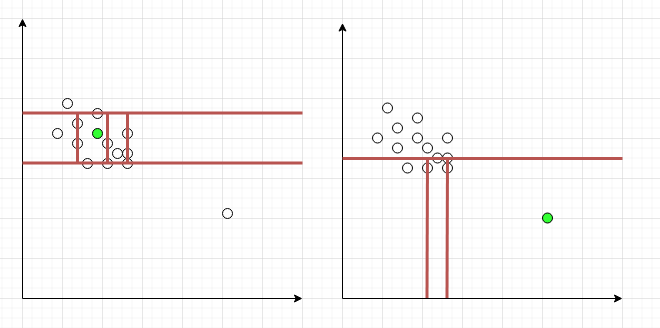
\includegraphics[width=0.9\textwidth]{Pictures/Sprint_4/isolation_forrest.png}
    \caption{Random cuts are performed until the point of interest is isolated (colored green). }
    \label{fig:iso}
\end{figure}

\noindent
The algorithm gives an anomaly score to every point. The point score is given by counting the number of random cuts required to isolate the point from all other points completely. In theory, this count should be lower for anomaly points, as illustrated in Figure \ref{fig:iso}. The algorithm is fast as it removes roughly half the remaining points at each cut.

The recursive nature of the cuts means that it can be represented by a tree structure where the number of cuts is equivalent to the length of a path from the root node to the terminating node. Averaging this path length over multiple random trees results in a better anomaly score\cite{isolation_forest}.

The algorithm is fast and works well on multidimensional data but also suffers from potentially bad accuracy as there can potentially be many false positives, especially if the anomaly threshold is not carefully set.

\subsection{Local Outlier Factor}
\gls{lof} is an algorithm used to find anomalies using an algorithm to find "local" anomalies first described in \cite{lof}. The idea is that anomalies are not only found globally, but also locally in clusters of data.

\begin{figure}[htbp]
    \centering
    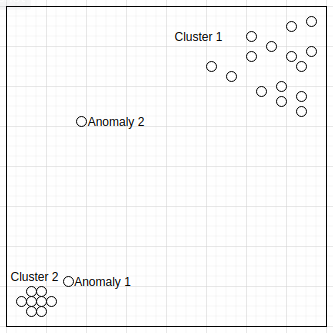
\includegraphics[width=0.4\textwidth]{Pictures/Sprint_4/lof.png}
    \caption{Local anomalies are looked at, instead of global anomalies.}
    \label{fig:lof}
\end{figure}

\noindent 
The algorithm looks for anomalies by looking at how many objects $p$, a specific object $o$, have a distance to less than the distance from $o$ to an object $k$, or the $k$-distance. If an object's distance to the object $o$, is less than the $k$-distance, it is part of the $k$-distance neighborhood of $o$, and part of the $k$-nearest neighbors.

As \gls{lof} has to look at local anomalies, a threshold for density can not be specified. As Figure \ref{fig:lof} shows, Anomaly one would not be considered an anomaly, if the density threshold was set not to specify Cluster one as anomalies. Instead of having a density threshold, it is necessary to compare the densities of different sets of objects. \gls{lof}, therefore, has to determine the density of clusters dynamically.

Because it has to determine the density of clusters dynamically, it is slower than \gls{iso}, but is more accurate in most cases.
\section{Network Evaluation}
When evaluating the network we will use a subset of our available datasets. Out of 62 datasets containing real-world univariate data we randomly choose 10 datasets. Of the 100 synthetic univariate datasets we also randomly choose ten datasets. Furthermore, out of the seven real-world multivariate datasets, we randomly choose two for evaluation. This is done to limit the amount of results to compare. \newline

\noindent
Table \ref{tab:datasets} shows the randomly chosen datasets. For every dataset we train five models. Training multiple models for every dataset allow us to ensure the result is consistent. The total amount of models produced will be 110 which should yield sufficient data for a good overall evaluation.

\bgroup
\def\arraystretch{1.8}
\begin{table}[htbp]
    \centering
    \begin{tabular}{| m{3cm} | m{3cm} | m{3cm} |}
        \hline
        \textbf{Synthetic} & \textbf{Real} & \textbf{Multivariate} \\
        \hline
        Synthetic\_12 & Real\_1 & chfdb\_chf01\_275 \\
        \hline
        Synthetic\_28 & Real\_19 & ltstdb\_20221\_43 \\
        \hline
        Synthetic\_30 & Real\_21 & ~ \\
        \hline
        Synthetic\_33 & Real\_25 & ~ \\
        \hline
        Synthetic\_37 & Real\_26 & ~ \\
        \hline
        Synthetic\_54 & Real\_27 & ~ \\
        \hline
        Synthetic\_70 & Real\_48 & ~ \\
        \hline
        Synthetic\_73 & Real\_55 & ~ \\
        \hline
        Synthetic\_91 & Real\_56 & ~ \\
        \hline
        Synthetic\_94 & Real\_62 & ~ \\
        \hline
    \end{tabular}
    \caption{Datasets used in the evaluation.}
    \label{tab:datasets}
\end{table}
\egroup

\FloatBarrier
\subsection{Baseline Results}
The results from \gls{iso} and \gls{lof} are shown in Table \ref{tab:baseline}. The results of the Isolation Forest show that all of the anomalies have been correctly labeled. However, the precision is very low, which means that the algorithm produces a lot of false positives. The low precision limits the usability of the prediction since the false positives obscure the true positives. \Gls{lof} performs better than (or equal) \gls{iso} in every metric. The recall is the same, however, the precision is higher and, therefore, fewer false positives. The higher precision makes \gls{lof} prediction more useful than \gls{iso} since there will be fewer false positives to obscure the true positives.

\begin{table}[htbp]
    \centering
    \begin{tabular}{|l|l|l|l|l|}
        \hline
        Catagory & Algorithm            & F1       & Precision & Recall \\ \hline
        Real     & Isolation Forest     & 0.199405 & 0.132799  & 1.0    \\ \hline
        Synth    & Isolation Forest     & 0.012255 & 0.006181  & 1.0    \\ \hline
        ECG      & Isolation Forest     & 0.359282 & 0.225992  & 1.0    \\ \hline
        Real     & Local Outlier Factor & 0.626562 & 0.499859  & 1.0    \\ \hline
        Synth    & Local Outlier Factor & 0.490043 & 0.380289  & 1.0    \\ \hline
        ECG      & Local Outlier Factor & 0.763543 & 0.625457  & 1.0    \\ \hline
    \end{tabular}
    \caption{Mean values for \gls{iso} and \gls{lof} for different types datasets.}\label{tab:baseline}
\end{table}

\noindent
We did not tune any parameters and left them as \glspl{scikit-learn} default. It is expected that better results can be achieved with more tuning. 


\subsection{RVAE result}
sfsdf
\section{Sprint Review} \label{sprint_4_review}
In this sprint we tested the service. We also evaluated on the network and baselines.
We used multiple randomly chosen datasets to get a broad range of examples to test the network on. We resolved the problem of stochasticicty by performing 
\phantomsection
\newpage
\chapter{Collaboration}
This chapter is dedicated to documenting the collaboration that took place during this project, both as part of the super-group, inter-group, and \gls{its} related collaborations.
\FloatBarrier
\oldsection*{Time Series Interface}
The input/output standard for time series data was accepted: 25th of March 2020 in a super-group meeting. The idea is that all the services that work with time-series data should be compatible with each other. The standard would allow for more interesting analytical options. It should be possible to chain different services together as long as they share a common interface. There were multiple meetings and design considerations to make the interface simple and useful.
SW602F20 took on the responsibility of implementing the necessary functionality to show the time series format in existing \gls{astep} chart-implementation. We choose to adopt this interface as we primarily work with time-series data. We took part in the initial discussion phase to make sure it would fit our project. We also tested and validated that our service works with this interface.

\FloatBarrier
\oldsection*{aSTEP Documentation}
In the first sprint, the \gls{astep} code-base was explored to understand the architecture and platform. There was some trouble getting proper, consistent documentation for the different services.
We proposed to use a Wiki type documentation system, and with help from the group, SW606F20 got it implemented in the interface. After multiple implementation options were considered, we chose Wiki.js \cite{wikijs} due to the modern look and simple deployment with \gls{docker}. It now includes both \gls{rfc}-list, meeting summaries, FAQ, server help, and service documentation. It makes all documentation for every \gls{astep} related activity available in one place. Our group collaborated with group SW603F20 to improve the documentation for \gls{kubernetes} in the Wiki.
\FloatBarrier
\oldsection*{Server Management}
It was chosen that one person from each group should take part in the server group, which made it possible for every group to get access to the server through their chosen server person. This made the server responsibility more scattered and avoided expertise islands.

A chatroom only accessible to the server group members was created, here they could share tips and collaborate on common server issues. This proved useful multiple times in various scenarios like:

\begin{itemize}
    \item Crashed Services
    \item Full disk/Resource limits
    \item Updating \gls{kubernetes}/\gls{gitlab}/Ubuntu
    \item Database management
    \item Reinstalling/configuring applications
\end{itemize}

\noindent
We also collaborated with \gls{its} on several occasions with varying success. Collaboration is needed since they control root access to the \gls{astep} servers. 

\FloatBarrier
\oldsection*{Tools}
The tools we used to collaborate are not that different from previous \gls{astep} groups as we took their advice on many of them.

\subsection*{Communication}
Most of the communication was organized on discord. Communication through discord proved beneficial when COVID-19 restrictions send everyone home. Discord has a proper voice channel implementation, and we used this tool in four areas for collaboration.
 
\begin{itemize}
     \item Supervisor meetings
     \item Group discussions
     \item Server group Collaborations
     \item Super group meetings
\end{itemize}

\subsection*{Version control}
Just as the \gls{astep} groups before us, we used the \gls{gitlab} server as a version control system. It now contains code from 2016 to 2020, and serves as shared repository for legacy services and archival of source code.

\Gls{gitlab} is set up with \gls{cicd} using a build server and a \gls{kubernetes} cluster. It works out of the box with simple hello world projects. We found this combination encourages collaboration between groups as we are developing for \gls{astep} on a shared platform.

\subsection*{Deployment}
We kept the \gls{kubernetes} servers as they seem to work well. It allows us to integrate with \gls{gitlab} and perform \gls{cicd}, besides a few updates and configuration changes it works largely the same, we found this made collaboration easy as a recent version was always live on \gls{astep} for testing. Collaborating when maintaining \gls{kubernetes} was easy as multiple users could use their login to control \gls{kubernetes} simultaneously.

\phantomsection
\newpage
\chapter{Reflections}
In this chapter we will share some overall reflections we have on the project, like a 'sprint retrospective' for 4 sprints combined. It is hoped that it might provide future student-projects, in \gls{astep}, with some insight into what could be done differently.
\FloatBarrier
\oldsection*{Collaboration}

\subsection*{Documentation}
The wiki now contains documentation for every \gls{astep} related activity. There is however, a glaring issue with the current kind of deployment. If \gls{kubernetes} goes down or is over-provisioned, the wiki will get inaccessible. The documentation for starting \gls{kubernetes} is placed in \emph{the wiki} in 'FAQ' and 'server help guides' wiki pages.
It could potentially be solved by setting better eviction policies in \gls{kubernetes} so the wiki stays up, or move the wiki to another kind of deployment altogether.

\subsection*{Communication}
While COVID-19 certainly hindered productivity, it could have been worse if shared voice channels were not accessible. We recommend a similar setup to Discord for future \gls{astep} teams, with possible alternatives as Slack and Microsoft Teams.

We would still strongly recommend physical meetings when possible, as that results in the fastest solutions and best learning experiences for us. 

\subsection*{Servers and \gls{its}}
The servers require some maintenance as they are quite low on some resources like disk space. We requested more resources to the server from \gls{its}. The request was however, denied.


\subsection*{Resources}
\gls{its}  opinion is that since some servers still have unused resources, we should use those first, which is fair but impractical. 
It would require extensive symlinking/networking to utilize separate partitions or other servers, a better solution is to migrate the troubled workload to a bigger host, and let \gls{its} reclaim the smaller host, currently the \gls{kubernetes} nodes use symlink tricks to utilize attached storage volumes which is not ideal.
For future \gls{astep} teams, we recommend telling \gls{its} that a bigger server is needed, do the migration and give the old (smaller) server back to \gls{its} as it seems simpler than explaining the true nature of the resource shortage, especially if the communication is conducted over email.

\subsection*{Authentication}
\gls{its} handles server credentials and we urge future \gls{astep} groups to hold on to as many credentials as possible and limit the reliance on \gls{its} which includes getting sudo rights to the servers to all the people that need it as early as possible, our group only got access after weeks of waiting, that slowed down debugging on docker related issues as we could not get the logs from the server.
We suggest limiting the number of people with sudo rights to one person per group as more poses risks, but fewer significantly increase reliance on other groups when debugging \gls{docker} issues.

\subsection*{Maintenance}
\gls{its} performs rudimentary server maintenance and virus detection but nothing more. Cleaning, updating, and rebooting is the \gls{astep} team's responsibility. It is especially important to empty \gls{docker} container registries often as they use many resources. The server group created a CRON-job that runs every night because the server got filled quickly during peak deployment days. 
\FloatBarrier
\oldsection*{Risk management}
\FloatBarrier
\oldsection*{Super meetings}

\label{LastPageLabel}

% To end the parts.
\bookmarksetup{startatroot}
\addtocontents{toc}{\bigskip}

% Bibliography.
\clearpage
\cleardoublepage
\phantomsection\addcontentsline{toc}{chapter}{Bibliography}
\label{bibliography}
\renewcommand\bibname{Bibliography}
\printbibliography{}
\clearpage{}
\ohead{{\MakeUppercase\leftmark}\rightmark}

% Appendix
\begin{appendices}
\phantomsection
\chapter{Risk Item Checklist} \label{app:A}
\bgroup 
\def\arraystretch{2}
\begin{table}[htbp]
    \begin{tabular}{| m{45mm} | l | l | l | m{50mm} |}
        \hline
        \textbf{Risk} & \textbf{P(r)} & \textbf{L(r)} & \textbf{E(r)} & \textbf{Consequence} \\
        \hline
        Server goes down. & 0.15 & 8 & 1.2 & \makecell[l]{Reduced productivity. \\ Loss of control.} \\
        \hline
        Inter group disagreement. & 0.9 & 3 & 2.7 & More time used in meetings. Work stalled until agreement. \\
        \hline
        Project dependencies not delivered on time. & 0.05 & 3 & 0.15 & \makecell[l]{Work is stalled. \\ More collaboration required.} \\
        \hline
        Unrealistic project scope. & 0.3 & 20 & 6 & \makecell[l]{Increased workload. Project \\ may fail to meet requirements.} \\
        \hline
        \makecell[l]{Technical debt from \\ legacy code.} & 0.4 & 3 & 1.2 & Time spent improving legacy code. \\
        \hline
        \makecell[l]{Extended absence of \\ group members.} & 0.6 & 2 & 1.2 & Increased workload for rest of group. \\
        \hline
        \makecell[l]{Extended time spent on \\ research.} & 0.8 & 5 & 4 & More time used before developing anything. \\
        \hline
        \makecell[l]{Spend too much time on \\ minor details} & 0.3 & 2 & 0.6 & Leads to wasted time, with no value behind. \\
        \hline
        \makecell[l]{Lack of experience with \\ servers} & 0.6 & 1 & 1.2 & Reduced productivity. More research time needed. \\
        \hline
        \makecell[l]{Lack of experience with \\ machine intelligence.} & 0.5 & 3 & 1.5 & More research time needed. \\
        \hline
        \makecell[l]{Group members leaving \\ the project} & 0.5 & 3 & 1.5 & Increased workload for rest of group. \\
        \hline
    \end{tabular}
    \caption{Unprioritized list of project risks.}
    \label{tab:risk_analysis}
\end{table}
\egroup
\phantomsection
\newpage
\chapter{RMMM Plan} \label{app:B}
\begin{figure}[htbp]
    \centering
    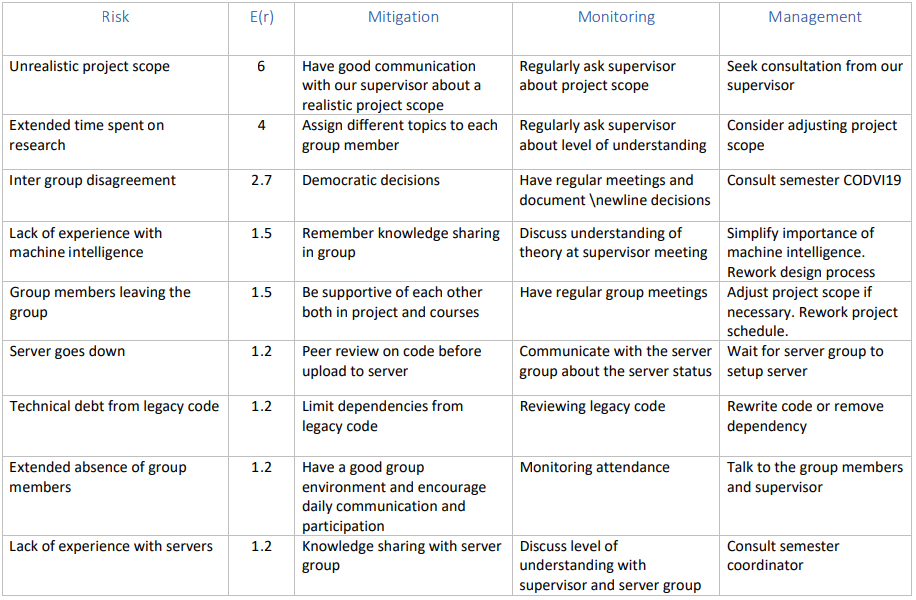
\includegraphics[scale=.635, angle=90]{Pictures/Sprint_1/RMM.png}
    \caption{Risk management plan.}
    \label{fig:my_label}
\end{figure}
\phantomsection
\newpage
% \chapter{Test}
\begin{center}
    \begin{longtable}[htbp]{| p{27mm} | l | p{27mm} | p{27mm} | p{27mm} |}
        \hline
        \textbf{Risk} & \textbf{E(r)} & \textbf{Mitigation} & \textbf{Monitoring} & \textbf{Management} \\ 
        \hline
        Unrealistic \newline project scope & 6 & Have good \newline communication \newline with our \newline supervisor about \newline a realistic project \newline scope & Regularly ask \newline supervisor about project scope & Seek \newline consultation from our \newline supervisor \\
        \hline
        Extended time \newline spent on \newline research & 4 & Assign different topics to each group member & Regularly ask supervisor about level of understanding. & Consider adjusting project scope. \\
        \hline
        Inter group \newline disagreement & 2.7 & Democratic \newline decisions & Have regular \newline meetings and \newline document \newline decisions & Consult semester coordinator \\
        \hline
        Lack of \newline experience with \newline machine intelligence. & 1.5 & Remember knowledge sharing in group. & Discuss understanding of theory at supervisor meetings. & Simplify importance of machine intelligence. Rework design process. \\
        \hline
        Group members leaving the group & 1.5 & Be supportive of each other both in project and courses. & Have regular \newline group meetings. & Adjust project \newline scope if necessary. Rework project schedule. \\
        \hline
        Server goes \newline down & 1.2 & Peer review on \newline code before \newline upload to server & Communicate \newline with the server \newline group about the \newline server status & Wait for server \newline group to setup \newline server \\
        \hline
        Technical debt \newline from legacy code & 1.2 & Limit \newline dependencies from legacy code & Reviewing legacy code & Rewrite code \newline or remove\newline dependency \\
        \hline
        Extended \newline absence of group \newline members & 1.2 & Have a good\newline group\newline environment and encourage daily communication and participation & Monitoring attendance & Talk to the group members and \newline supervisor \\
        \hline
        Lack of experience with servers & 1.2 & Knowledge sharing with server group. & Discuss level of understanding with supervisor and server group. & Consult semester coordinator. \\
        \hline
        \caption{Risk management plan.}
    \end{longtable}
\end{center}
% \phantomsection
% \newpage
\chapter{Experiment Parameters}\label{app:experiments}
\begin{table}[htbp]
\centering
\begin{tabular}{|c|c|c|c|c|c|c|c|c|}
\hline
\multicolumn{9}{|c|}{Batch Size Experiment}                                                                                                                                                                                                                                                                 \\ \hline
GRU & Dense & Window Size & LR   & \multicolumn{2}{c|}{\begin{tabular}[c]{@{}c@{}}Early Stopping\\ (patience, epsilon)\end{tabular}} & \multicolumn{2}{c|}{\begin{tabular}[c]{@{}c@{}}Learning rate decay\\ (decay rate, frequency)\end{tabular}} & \begin{tabular}[c]{@{}c@{}}KL-div\\ factor\end{tabular} \\ \hline
32  & 32    & 32          & 1e-3 & 100                                              & 0                                              & 0.8                                                  & 10                                                  & 0/off                                                   \\ \hline
\end{tabular}
\caption{Batch size experiment parameters}
\label{tab:exp-batchsize}
\end{table}
\phantomsection
\newpage
\end{appendices}

\end{myenv}
\end{document}